\documentclass[notes,11pt, aspectratio=169]{beamer}

\usepackage{pgfpages}
% These slides also contain speaker notes. You can print just the slides,
% just the notes, or both, depending on the setting below. Comment out the want
% you want.
\setbeameroption{hide notes} % Only slide
%\setbeameroption{show only notes} % Only notes
%\setbeameroption{show notes on second screen=right} % Both

\usepackage{helvet}
\usepackage[default]{lato}
\usepackage{array}
\usepackage{tgbonum}

\usepackage{tikz}
\usepackage{verbatim}
\setbeamertemplate{note page}{\pagecolor{yellow!5}\insertnote}
\usetikzlibrary{positioning}
\usetikzlibrary{snakes}
\usetikzlibrary{calc}
\usetikzlibrary{arrows}
\usetikzlibrary{decorations.markings}
\usetikzlibrary{shapes.misc}
\usetikzlibrary{matrix,shapes,arrows,fit,tikzmark}
\usepackage{amsmath}
\usepackage{mathpazo}
\usepackage{hyperref}
\usepackage{lipsum}
\usepackage{multimedia}
\usepackage{graphicx}
\usepackage{multirow}
\usepackage{graphicx}
\usepackage{dcolumn}
\usepackage{bbm}
\newcolumntype{d}[0]{D{.}{.}{5}}

\usepackage{changepage}
\usepackage{appendixnumberbeamer}
\newcommand{\beginbackup}{
   \newcounter{framenumbervorappendix}
   \setcounter{framenumbervorappendix}{\value{framenumber}}
   \setbeamertemplate{footline}
   {
     \leavevmode%
     \hline
     box{%
       \begin{beamercolorbox}[wd=\paperwidth,ht=2.25ex,dp=1ex,right]{footlinecolor}%
%         \insertframenumber  \hspace*{2ex} 
       \end{beamercolorbox}}%
     \vskip0pt%
   }
 }
\newcommand{\backupend}{
   \addtocounter{framenumbervorappendix}{-\value{framenumber}}
   \addtocounter{framenumber}{\value{framenumbervorappendix}} 
}


\usepackage{graphicx}
\usepackage[space]{grffile}
\usepackage{booktabs}
\newcommand\independent{\protect\mathpalette{\protect\independenT}{\perp}}
\def\independenT#1#2{\mathrel{\rlap{$#1#2$}\mkern2mu{#1#2}}}
\DeclareMathOperator{\Supp}{Supp}


\newtheorem{assN}{Assumption}
% These are my colors -- there are many like them, but these ones are mine.
\definecolor{blue}{RGB}{0,114,178}
\definecolor{red}{RGB}{213,94,0}
\definecolor{yellow}{RGB}{240,228,66}
\definecolor{green}{RGB}{0,158,115}

\hypersetup{
  colorlinks=false,
  linkbordercolor = {white},
  linkcolor = {blue}
}


%% I use a beige off white for my background
\definecolor{MyBackground}{RGB}{255,253,218}

%% Uncomment this if you want to change the background color to something else
%\setbeamercolor{background canvas}{bg=MyBackground}

%% Change the bg color to adjust your transition slide background color!
\newenvironment{transitionframe}{
  \setbeamercolor{background canvas}{bg=yellow}
  \begin{frame}}{
    \end{frame}
}

\setbeamercolor{frametitle}{fg=blue}
\setbeamercolor{title}{fg=black}
\setbeamertemplate{footline}[frame number]
\setbeamertemplate{navigation symbols}{} 
\setbeamertemplate{itemize items}{-}
\setbeamercolor{itemize item}{fg=blue}
\setbeamercolor{itemize subitem}{fg=blue}
\setbeamercolor{enumerate item}{fg=blue}
\setbeamercolor{enumerate subitem}{fg=blue}
\setbeamercolor{button}{bg=MyBackground,fg=blue,}



% If you like road maps, rather than having clutter at the top, have a roadmap show up at the end of each section 
% (and after your introduction)
% Uncomment this is if you want the roadmap!
% \AtBeginSection[]
% {
%    \begin{frame}
%        \frametitle{Roadmap of Talk}
%        \tableofcontents[currentsection]
%    \end{frame}
% }
\setbeamercolor{section in toc}{fg=blue}
\setbeamercolor{subsection in toc}{fg=red}
\setbeamersize{text margin left=1em,text margin right=1em} 

\newenvironment{wideitemize}{\itemize\addtolength{\itemsep}{10pt}}{\enditemize}

\usepackage{environ}
\NewEnviron{videoframe}[1]{
  \begin{frame}
    \vspace{-8pt}
    \begin{columns}[onlytextwidth, T] % align columns
      \begin{column}{.70\textwidth}
        \begin{minipage}[t][\textheight][t]
          {\dimexpr\textwidth}
          \vspace{8pt}
          \hspace{4pt} {\Large \sc \textcolor{blue}{#1}}
          \vspace{8pt}
          
          \BODY
        \end{minipage}
      \end{column}%
      \hfill%
      \begin{column}{.38\textwidth}
        \colorbox{green!20}{\begin{minipage}[t][1.2\textheight][t]
            {\dimexpr\textwidth}
            Face goes here
          \end{minipage}}
      \end{column}%
    \end{columns}
  \end{frame}
}

\title[]{\textcolor{blue}{Canonical Research Designs VII:\\ Regression
    Discontinuity II:\\ The Checklist}} \author[PGP]{}
\institute[FRBNY]{\small{\begin{tabular}{c}
                           Paul Goldsmith-Pinkham  \\
\end{tabular}}}

\date{\today}

\begin{document}

%%% TIKZ STUFF
\tikzset{   
        every picture/.style={remember picture,baseline},
        every node/.style={anchor=base,align=center,outer sep=1.5pt},
        every path/.style={thick},
        }
\newcommand\marktopleft[1]{%
    \tikz[overlay,remember picture] 
        \node (marker-#1-a) at (-.3em,.3em) {};%
}
\newcommand\markbottomright[2]{%
    \tikz[overlay,remember picture] 
        \node (marker-#1-b) at (0em,0em) {};%
}
\tikzstyle{every picture}+=[remember picture] 
\tikzstyle{mybox} =[draw=black, very thick, rectangle, inner sep=10pt, inner ysep=20pt]
\tikzstyle{fancytitle} =[draw=black,fill=red, text=white]
%%%% END TIKZ STUFF

% Title Slide
\begin{frame}
\maketitle
\end{frame}

\begin{frame}{Roadmap for Today}
  \begin{wideitemize}
  \item Last time: assumptions for RD, and estimation basics
  \item This time: how to implement RD, and checklist
    \begin{itemize}
    \item E.g., if I'm writing a paper on RD, what would I need to show?
    \end{itemize}
  \end{wideitemize}
\end{frame}

\begin{frame}{Running example}
    \begin{columns}[onlytextwidth, T] % align columns
      \begin{column}{.5\textwidth}
        \begin{wideitemize}
        \item Lee (2008) studies the impact of a Democrat winning on subsequent victory
        \item Running variable $Z$: vote share margin of victory
        \item $D$: winning election
        \item $Y$: Subsequent victory in an election
          \begin{itemize}
          \item<2-> $Y$: Subsequent candidacy in an election
          \item<3-> $Y$: Subsequent vote share in an election             
          \end{itemize}
        \end{wideitemize}
      \end{column}%
      \hfill%
      \begin{column}{.5\textwidth}
        \only<1>{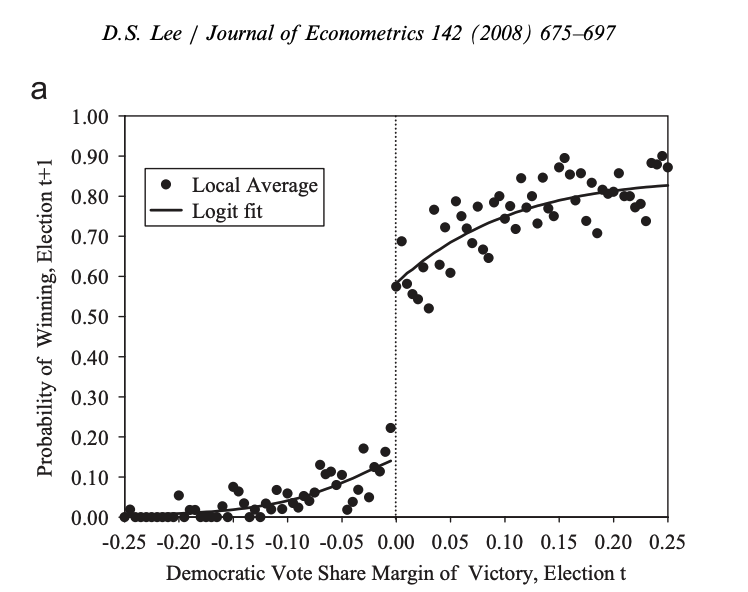
\includegraphics[width=\linewidth]{images/lee_1a.png}}
        \only<2>{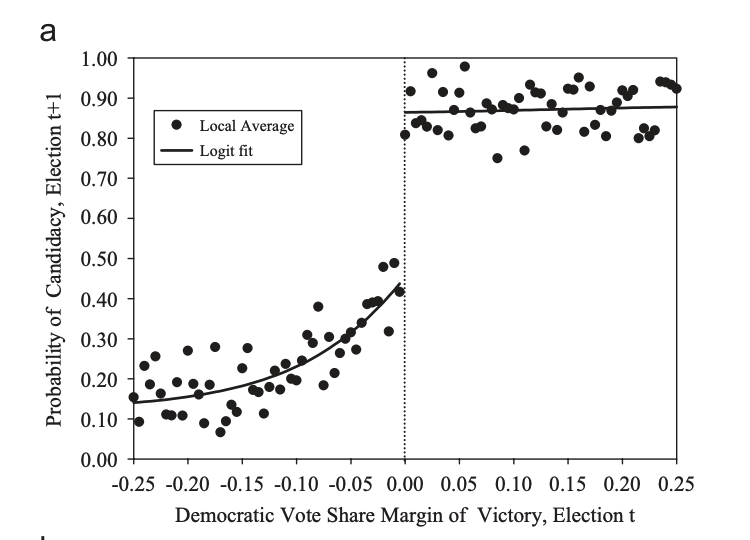
\includegraphics[width=\linewidth]{images/lee_1b.png}}
        \only<3>{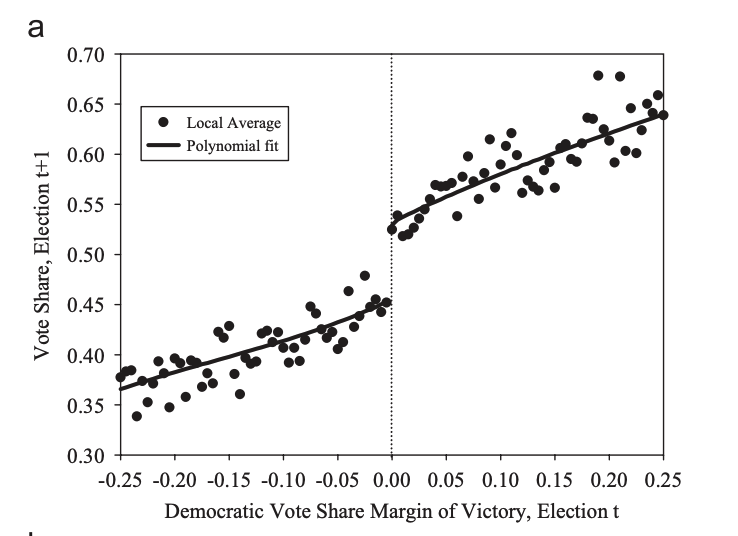
\includegraphics[width=\linewidth]{images/lee_1c.png}}                
      \end{column}%
    \end{columns}
\end{frame}

\begin{frame}{A checklist for how to support this analysis}
    \begin{columns}[onlytextwidth, T] % align columns
      \begin{column}{.9\textwidth}
        \begin{itemize}
        \item A graphical representation and test of ``balance'' and first stage (if fuzzy)
        \item Permutation test of characteristic at cutoff 
        \item The density of the forcing variable (Mcrary test)
        \item Placebo checks
        \item A graphical representation of the outcomes (what we've already seen)          
        \item Estimates based on optimal bandwidth choice and robust
          inference, using local linear analysis
          \begin{itemize}
          \item These decisions vary depending on running variable. If
            discrete running variable, need to account for
            discreteness (Kolesar and Rothe (2018))
          \item Should use local linear regression, and not global polynomials (Gelman and Imbens)
          \end{itemize}
        \item Robustness analysis along bandwidth choice (and other tuning parameters)
          \begin{itemize}
          \item Present this graphically
          \end{itemize}
        \end{itemize}
      \end{column}%
      \hfill%
      \begin{column}{.3\textwidth}
      \end{column}%
    \end{columns}
\end{frame}

\begin{frame}{Checking for balance}
  \begin{columns}[onlytextwidth, T] % align columns
    \begin{column}{.5\textwidth}
      \begin{wideitemize}
      \item Our identification strategy, like in all settings, is
        not inherently testable
      \item But, there are things that we can look at whether they
        are consistent with our hypothesis
      \item In Lee (2007), the most natural test is whether the
        cutoff in period $t$ affects the probability of victory in
        period $t-1$, the period before
      \item Other natural tests exist as well: looking for balance
        in outcomes that should not be affected by the treatment:
        \begin{itemize}
        \item predermined covariates
        \item things with no causal link 
        \end{itemize}
      \end{wideitemize}
    \end{column}%
    \hfill%
    \begin{column}{.5\textwidth}
      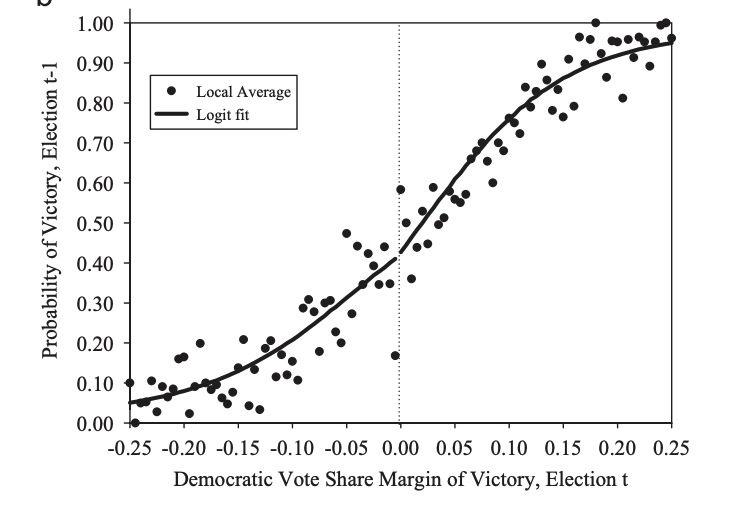
\includegraphics[width=\linewidth]{images/lee3b.png}
    \end{column}%
  \end{columns}
\end{frame}

\begin{frame}{A quick aside on graphical construction}
  \begin{columns}[onlytextwidth, T] % align columns
    \begin{column}{.5\textwidth}
      \begin{wideitemize}
      \item One of the most powerful aspects of regression
        discontinuity is the ability to present the results
        graphically. So what's the right approach?
      \item First, worth noting that the raw data is rarely informative without some amount of grouping
        \begin{itemize}
        \item Consider the main Lee (2008) result, with just raw data
        \end{itemize}
      \item Remarkably, you fact see a jump in the distribution in the data
        \begin{itemize}
        \item But the signal to noise ratio is low
        \end{itemize}
      \end{wideitemize}
    \end{column}%
    \hfill%
    \begin{column}{.5\textwidth}
      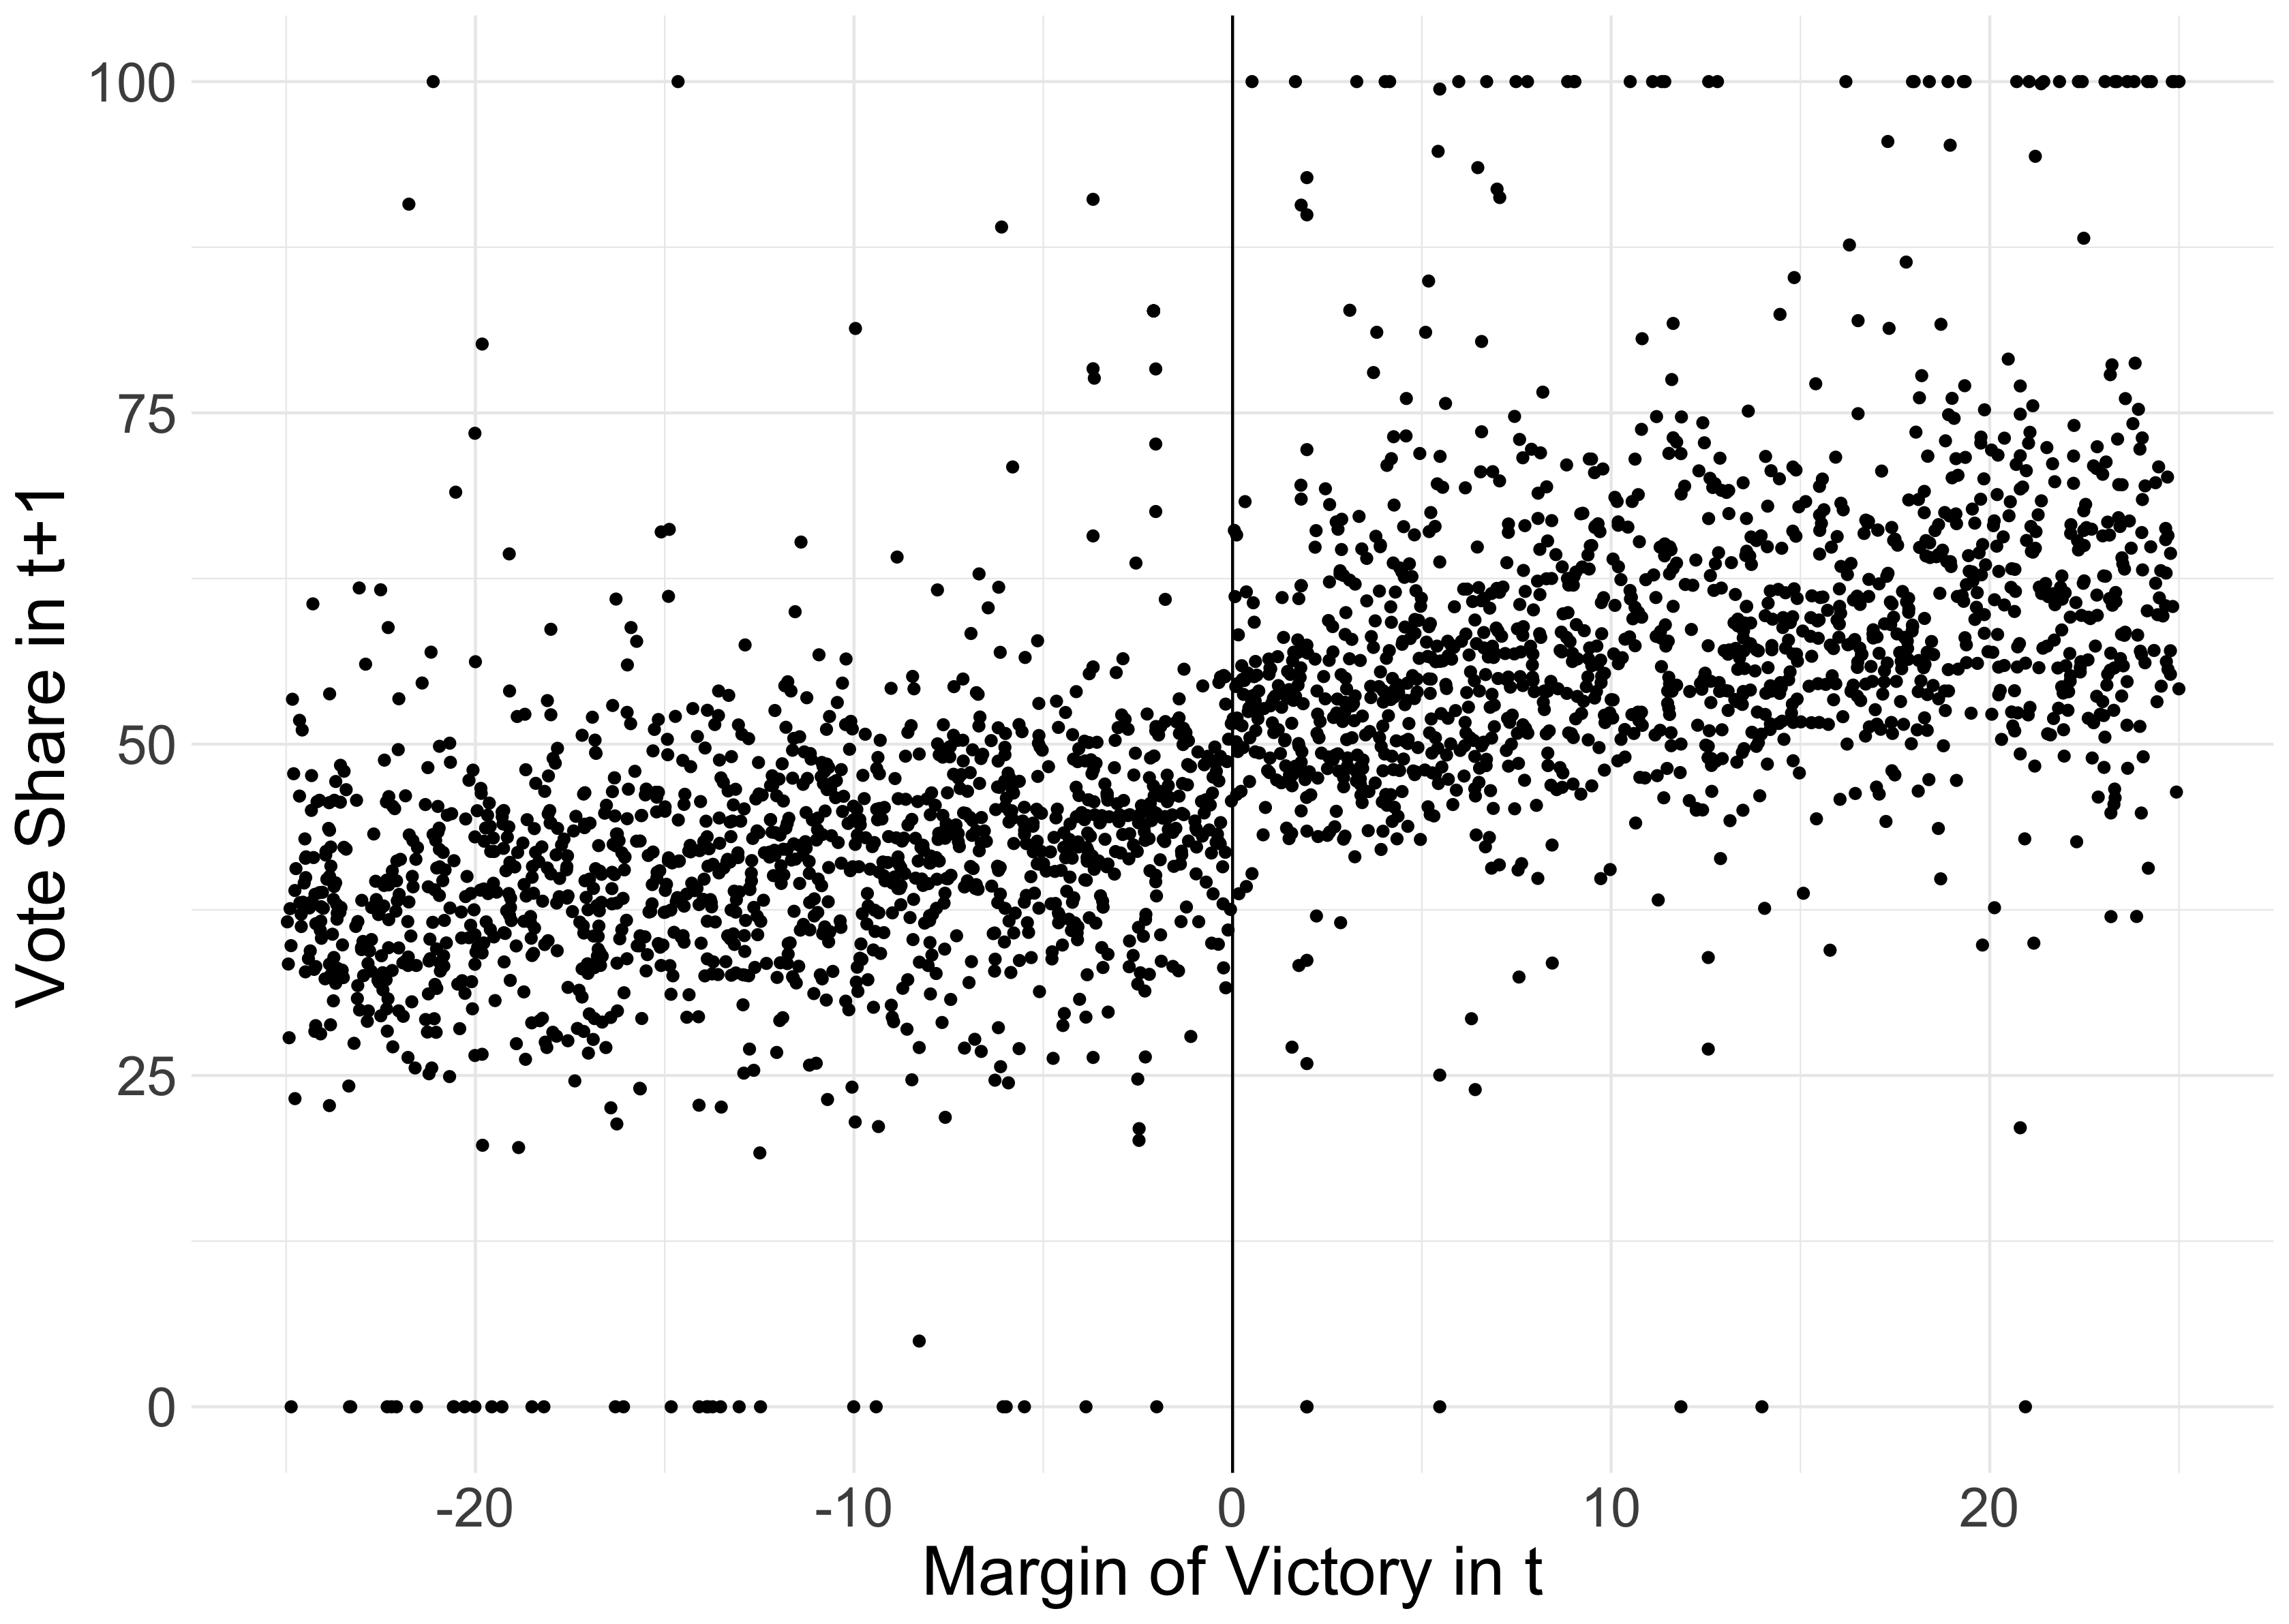
\includegraphics[width=\linewidth]{images/lee_rd_scatter.png}
    \end{column}%
  \end{columns}
\end{frame}

\begin{frame}{A quick aside on graphical construction}
  \begin{columns}[onlytextwidth, T] % align columns
    \begin{column}{.5\textwidth}
      \begin{wideitemize}
      \item Ideally, you would plot a version of the scatter plot, but
        focusing on means within binned areas
        \begin{itemize}
        \item This is exactly the intuition from binscatter, and a
          similar statistical problem
        \item How do we choose bins?
        \end{itemize}
      \item Simple first approach - equally spaced bins
        \begin{itemize}
        \item But how big?
        \item Lee (2008) chooses 0.5 percent bins
        \item But why does this look less compelling?
        \end{itemize}
      \end{wideitemize}
    \end{column}%
    \hfill%
    \begin{column}{.5\textwidth}
      \only<1>{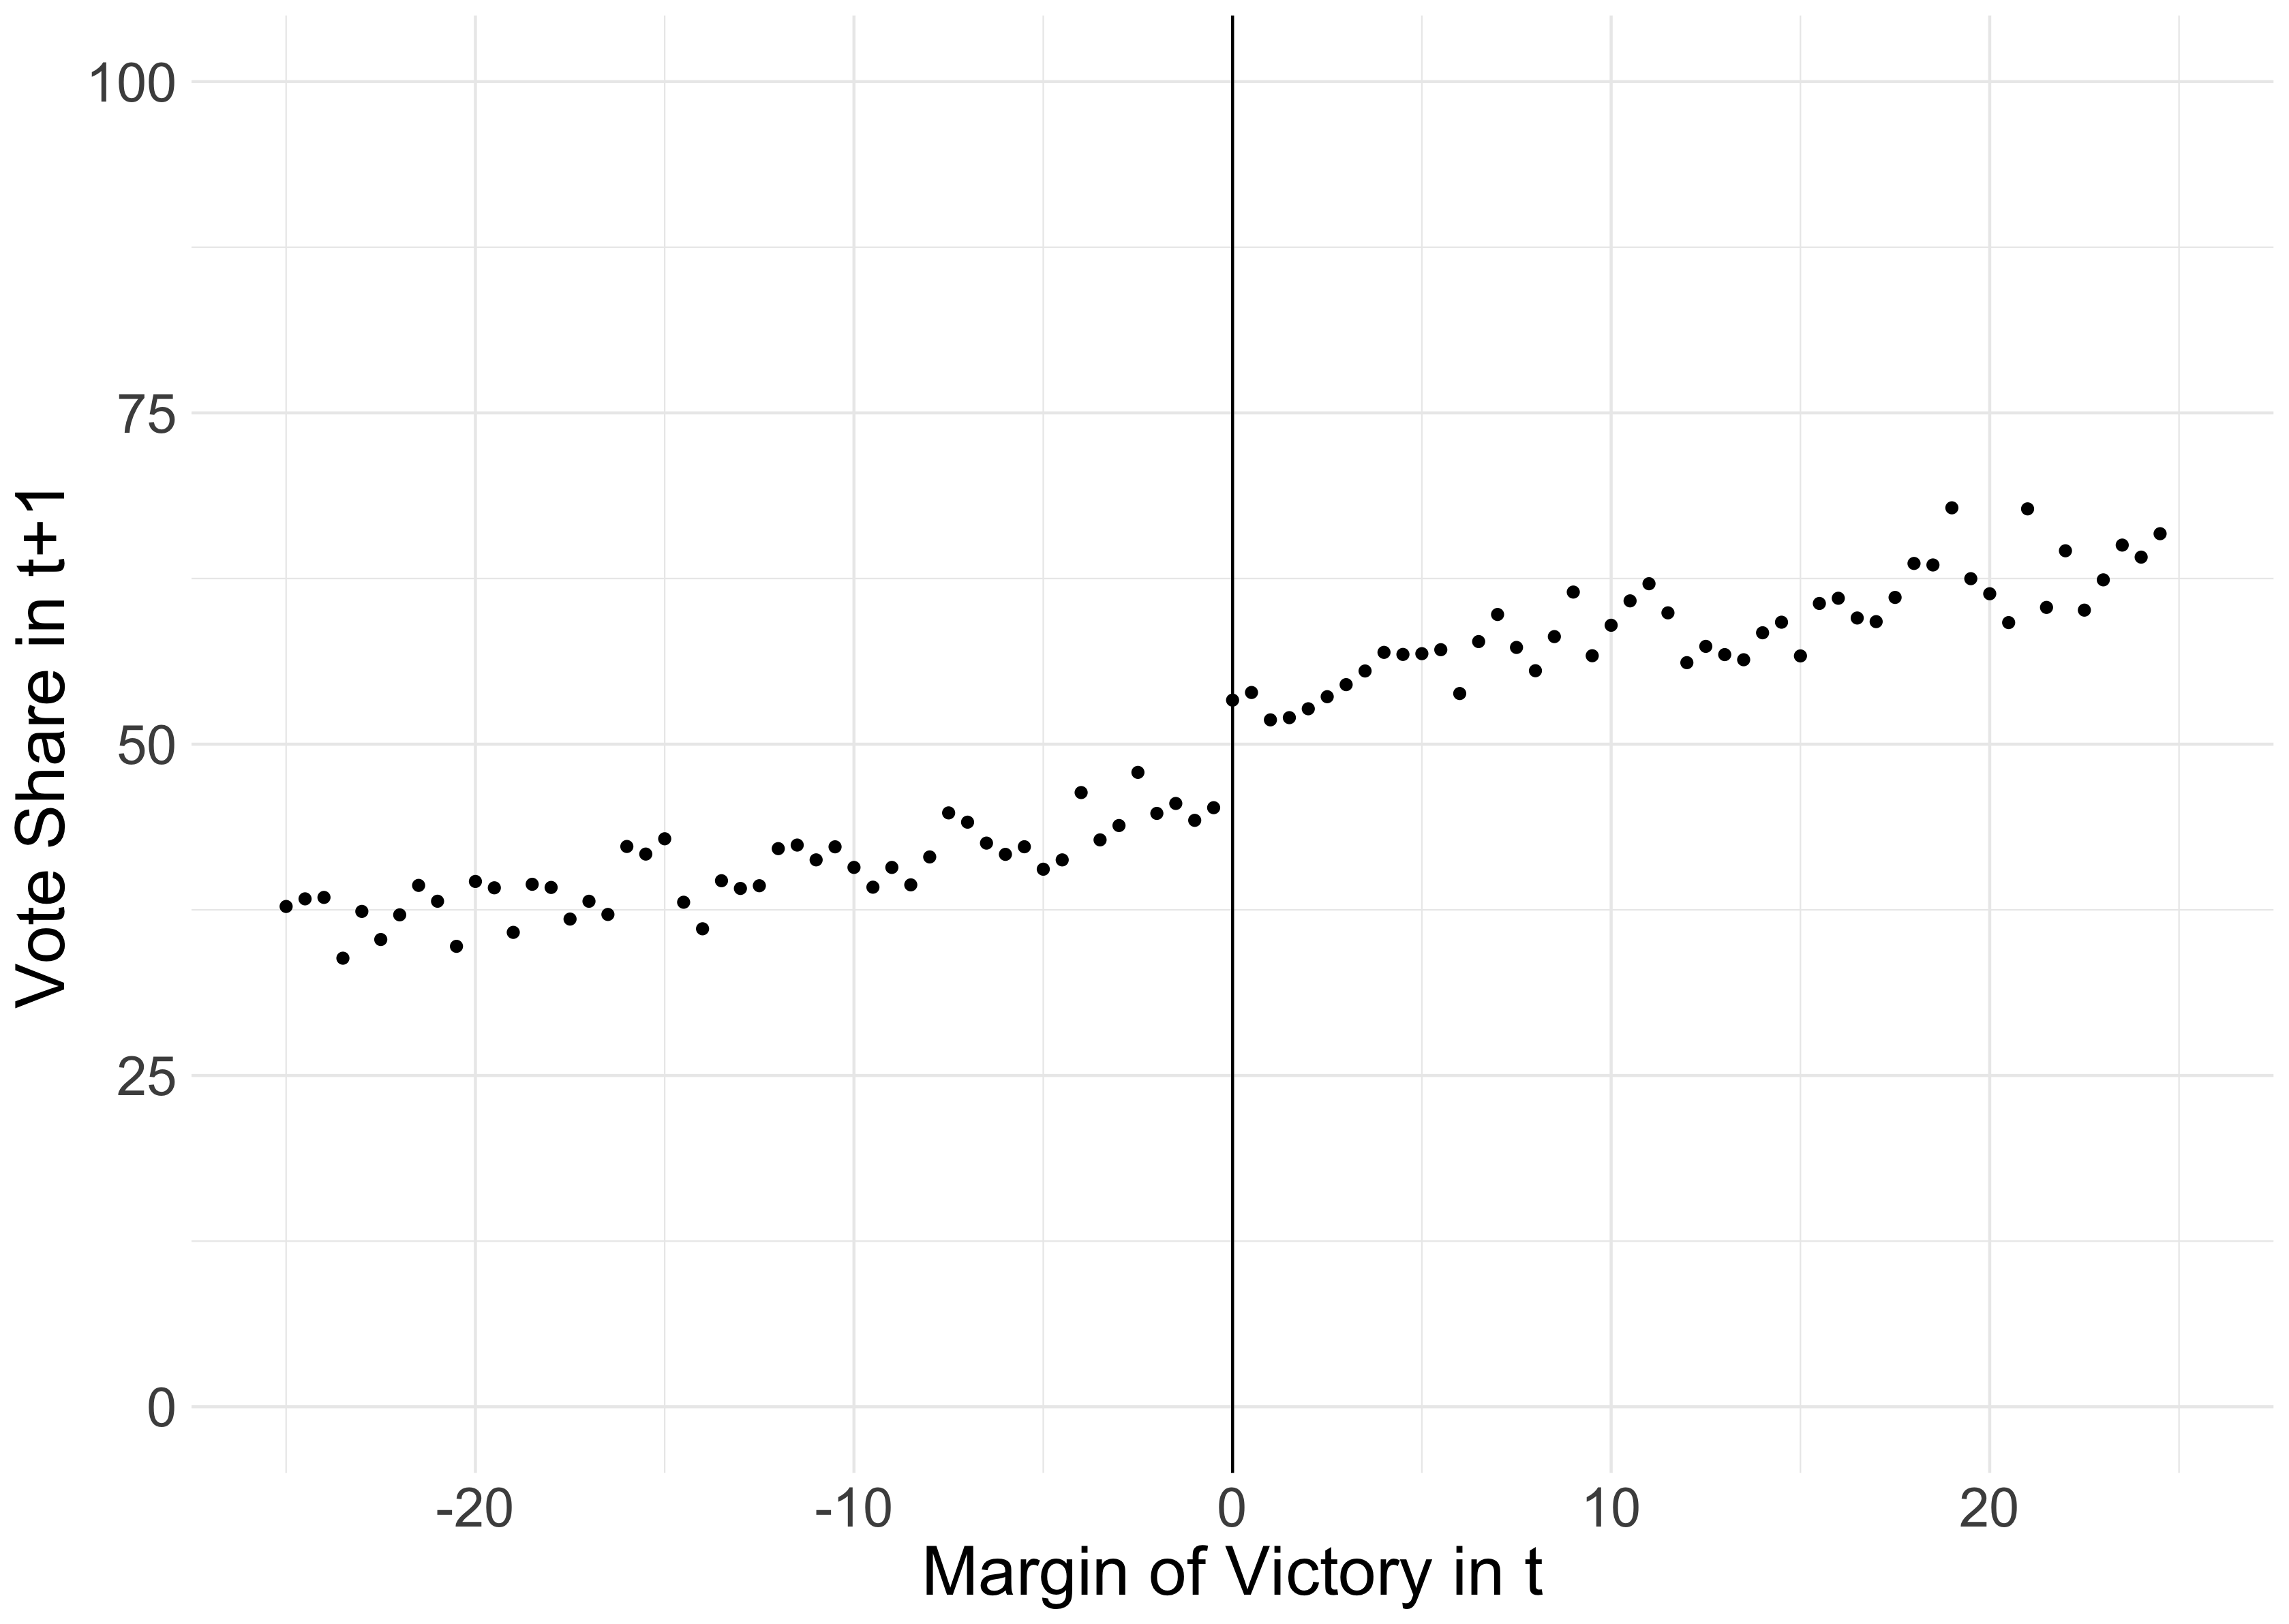
\includegraphics[width=\linewidth]{images/lee_rd_binscatter1.png}}
      \only<2>{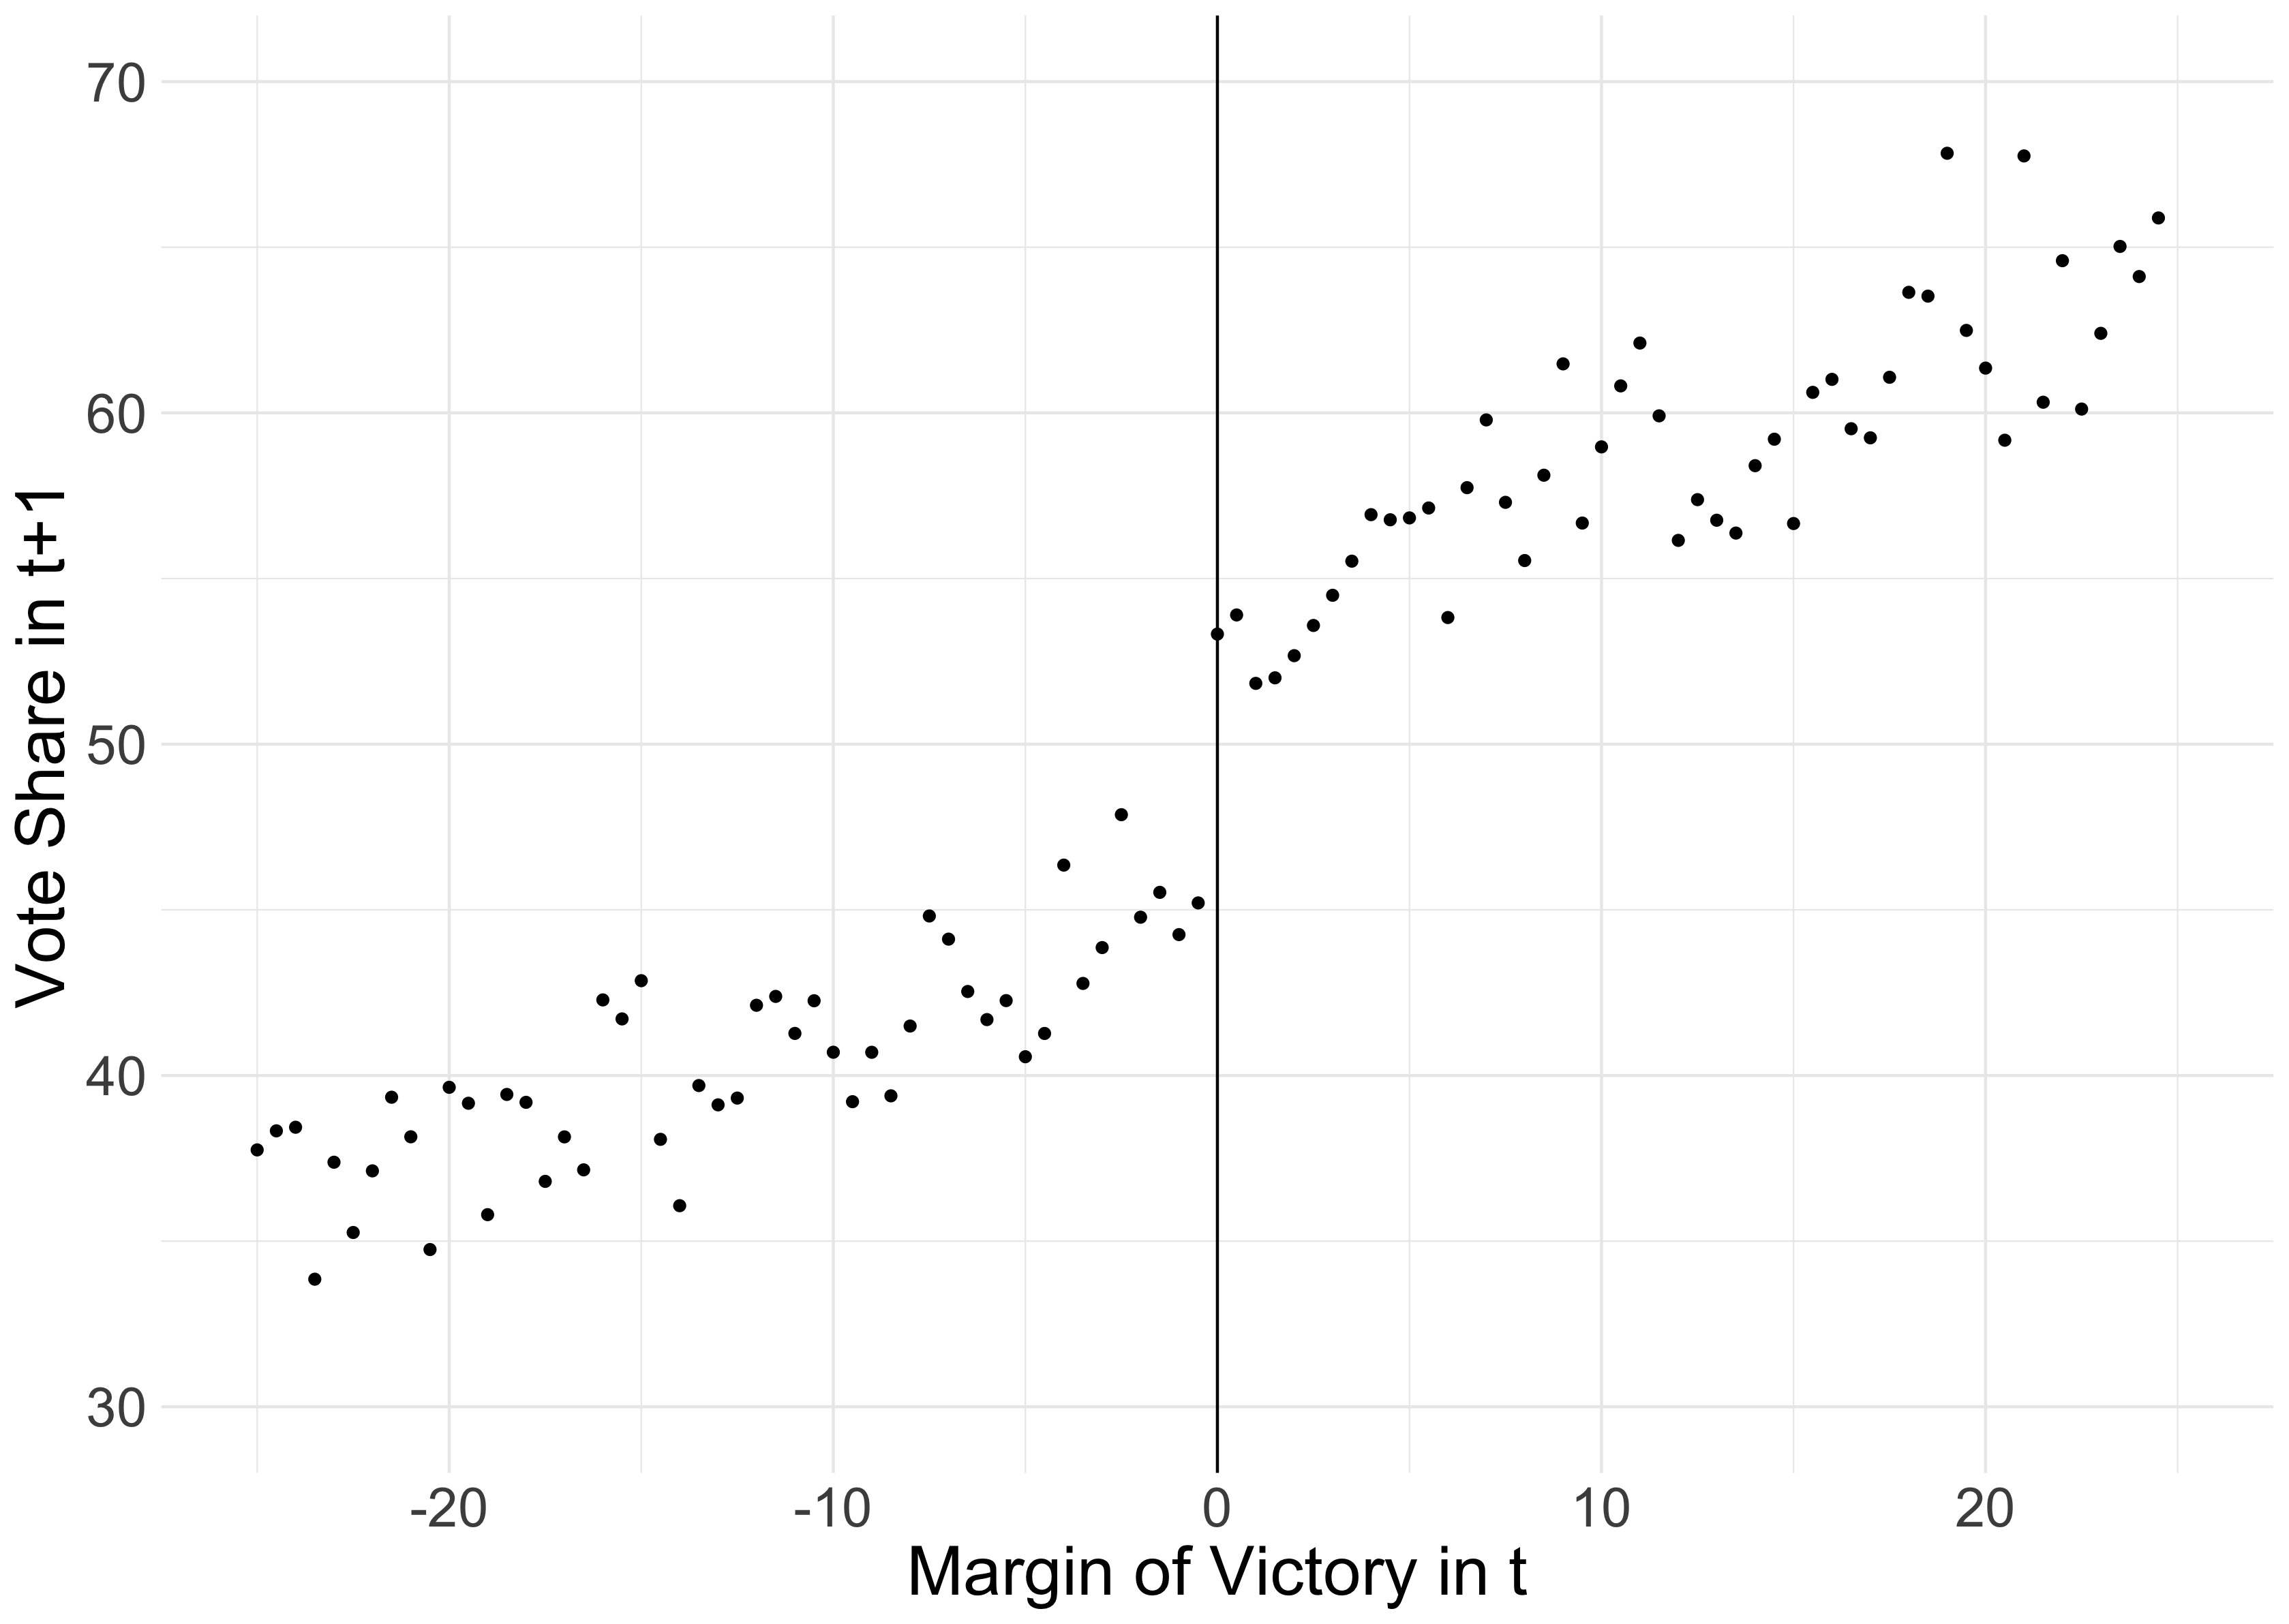
\includegraphics[width=\linewidth]{images/lee_rd_binscatter1b.png}      }
    \end{column}%
  \end{columns}
\end{frame}

\begin{frame}{A quick aside on graphical construction}
  \begin{columns}[onlytextwidth, T] % align columns
    \begin{column}{.5\textwidth}
      \begin{wideitemize}
      \item The choice is bin is non-trivial
      \item What does this look like with bins of 4 percent? 0.1 percent?
      \item<3-> As with our discussion of estimating non-parametric
        means, the trade-off in number of bins typically comes down to
        bias (more bins helps get closer to the ``true'' conditional
        means) and noise (less bins increases observations within
        bins, lowering the SE for a bin)
      \end{wideitemize}
    \end{column}%
    \hfill%
    \begin{column}{.5\textwidth}
      \only<1>{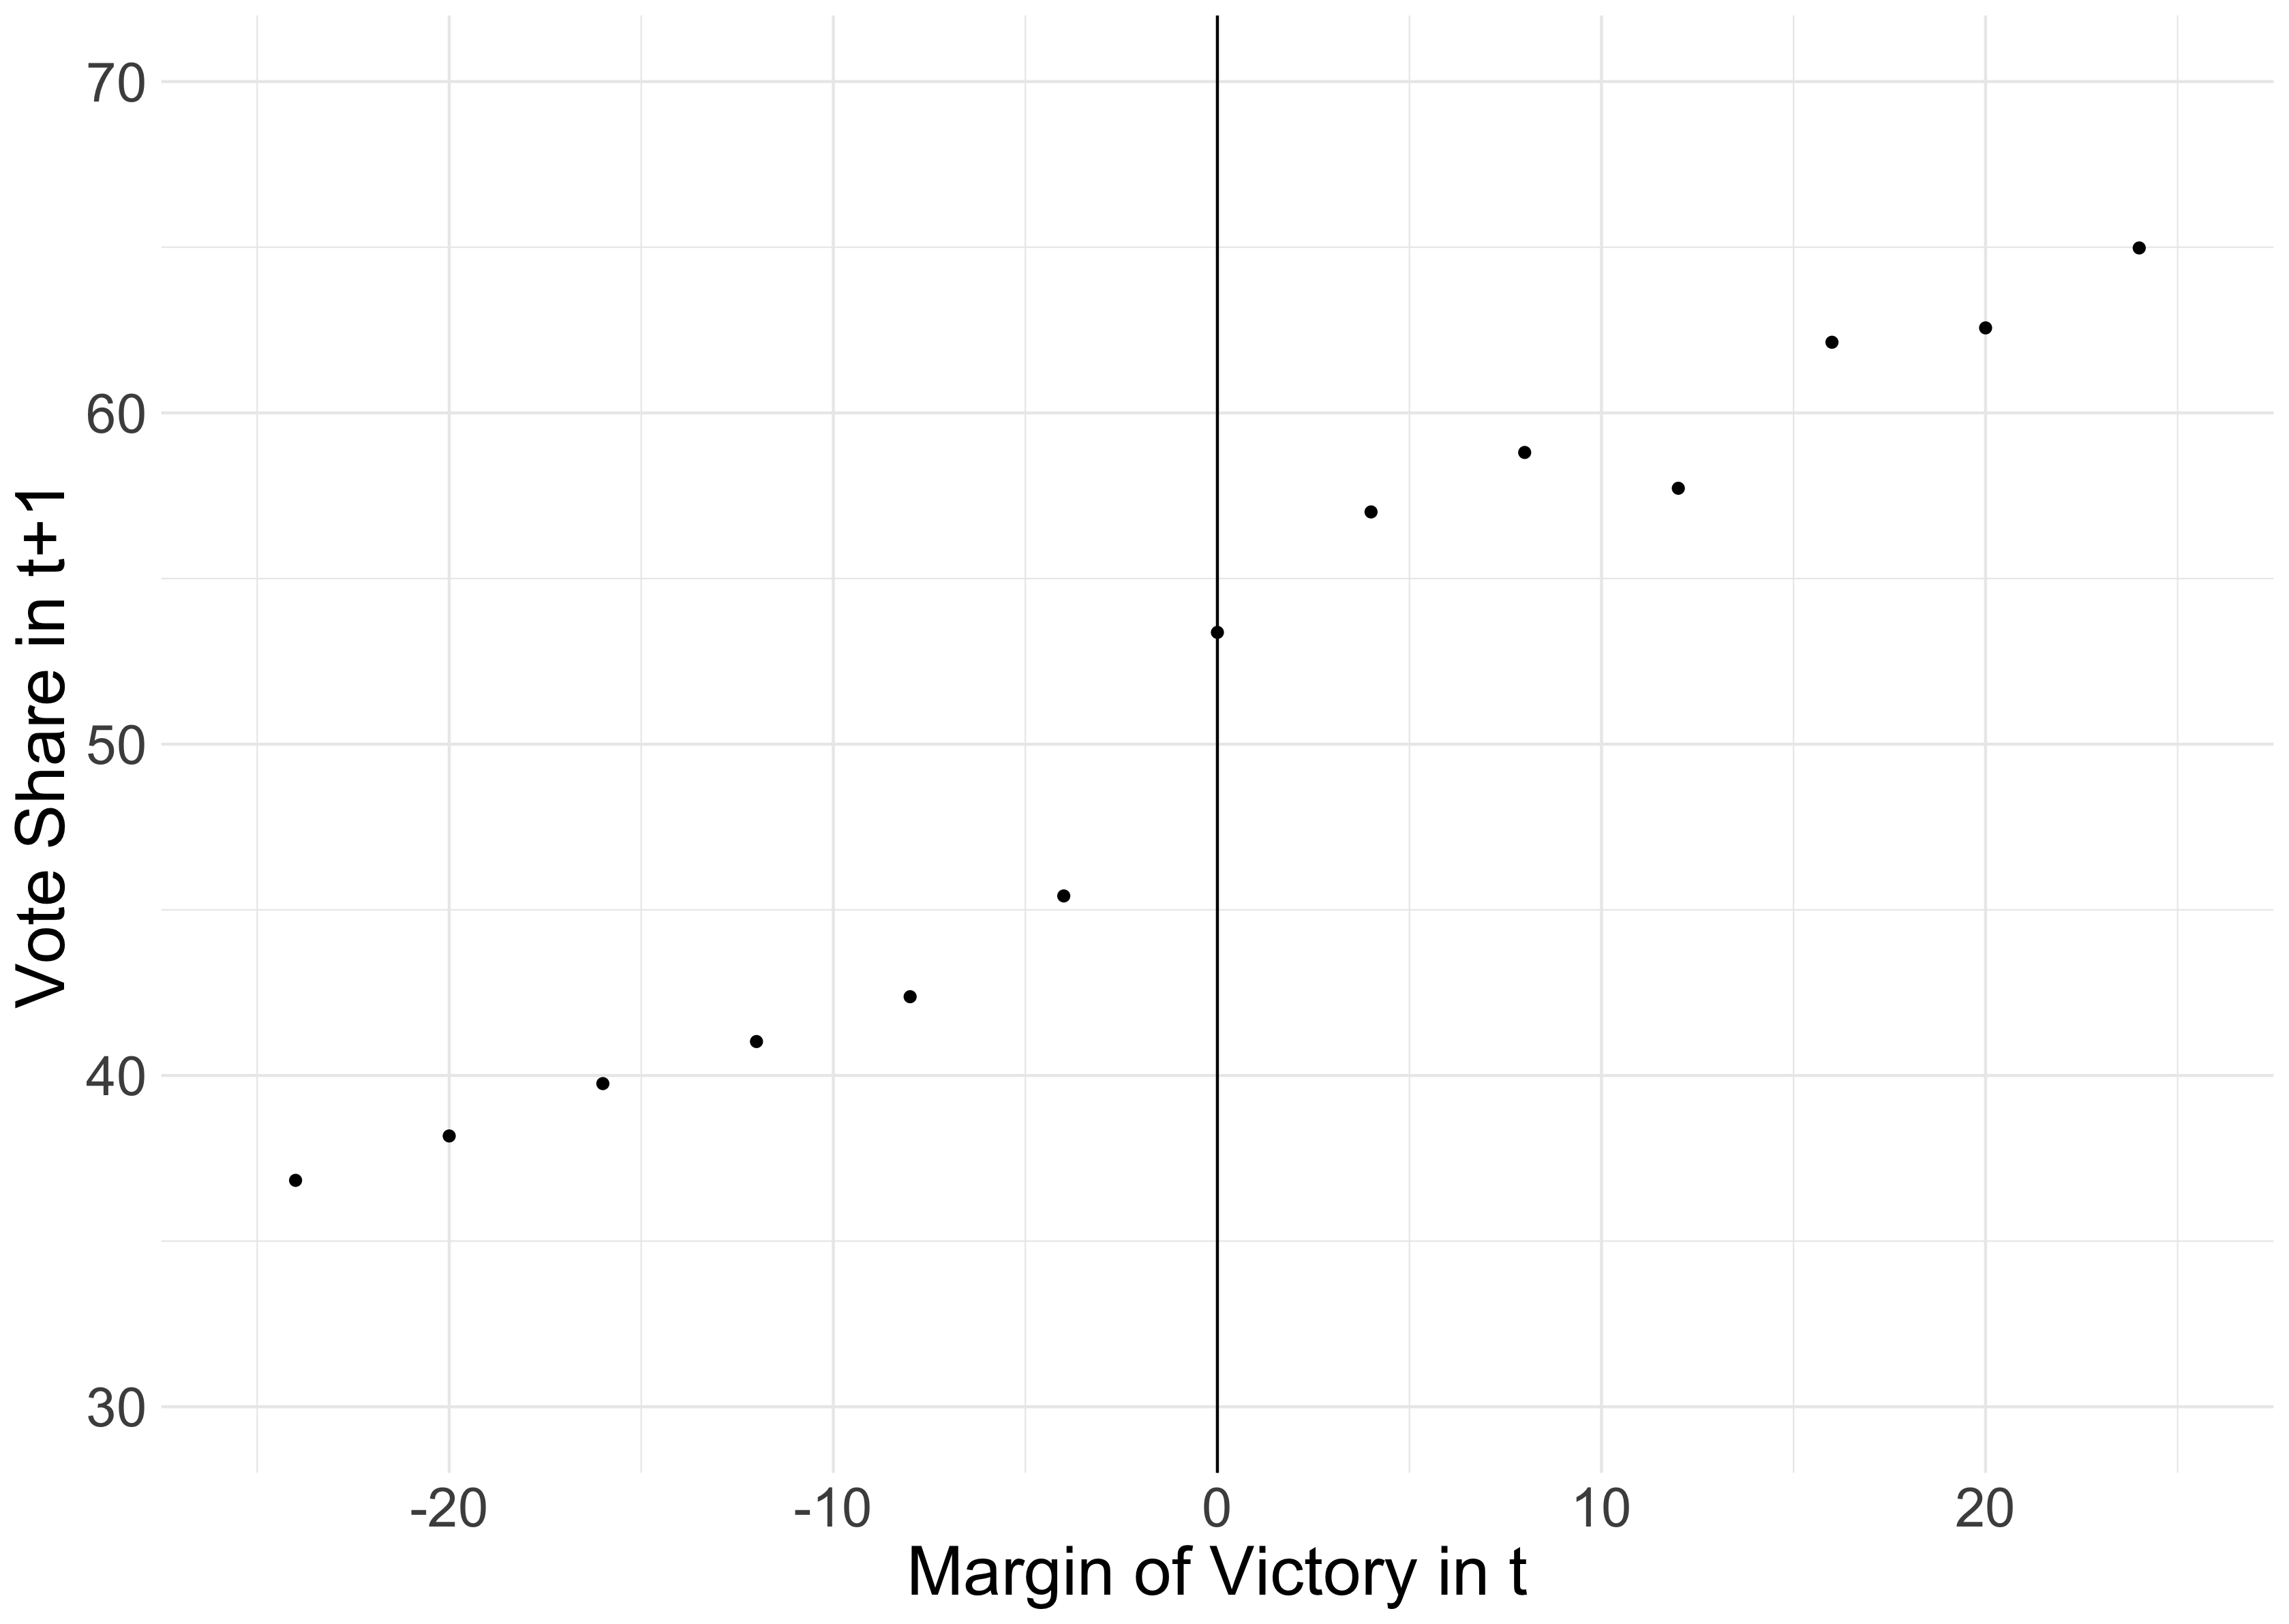
\includegraphics[width=\linewidth]{images/lee_rd_binscatter1d.png}}
      \only<2->{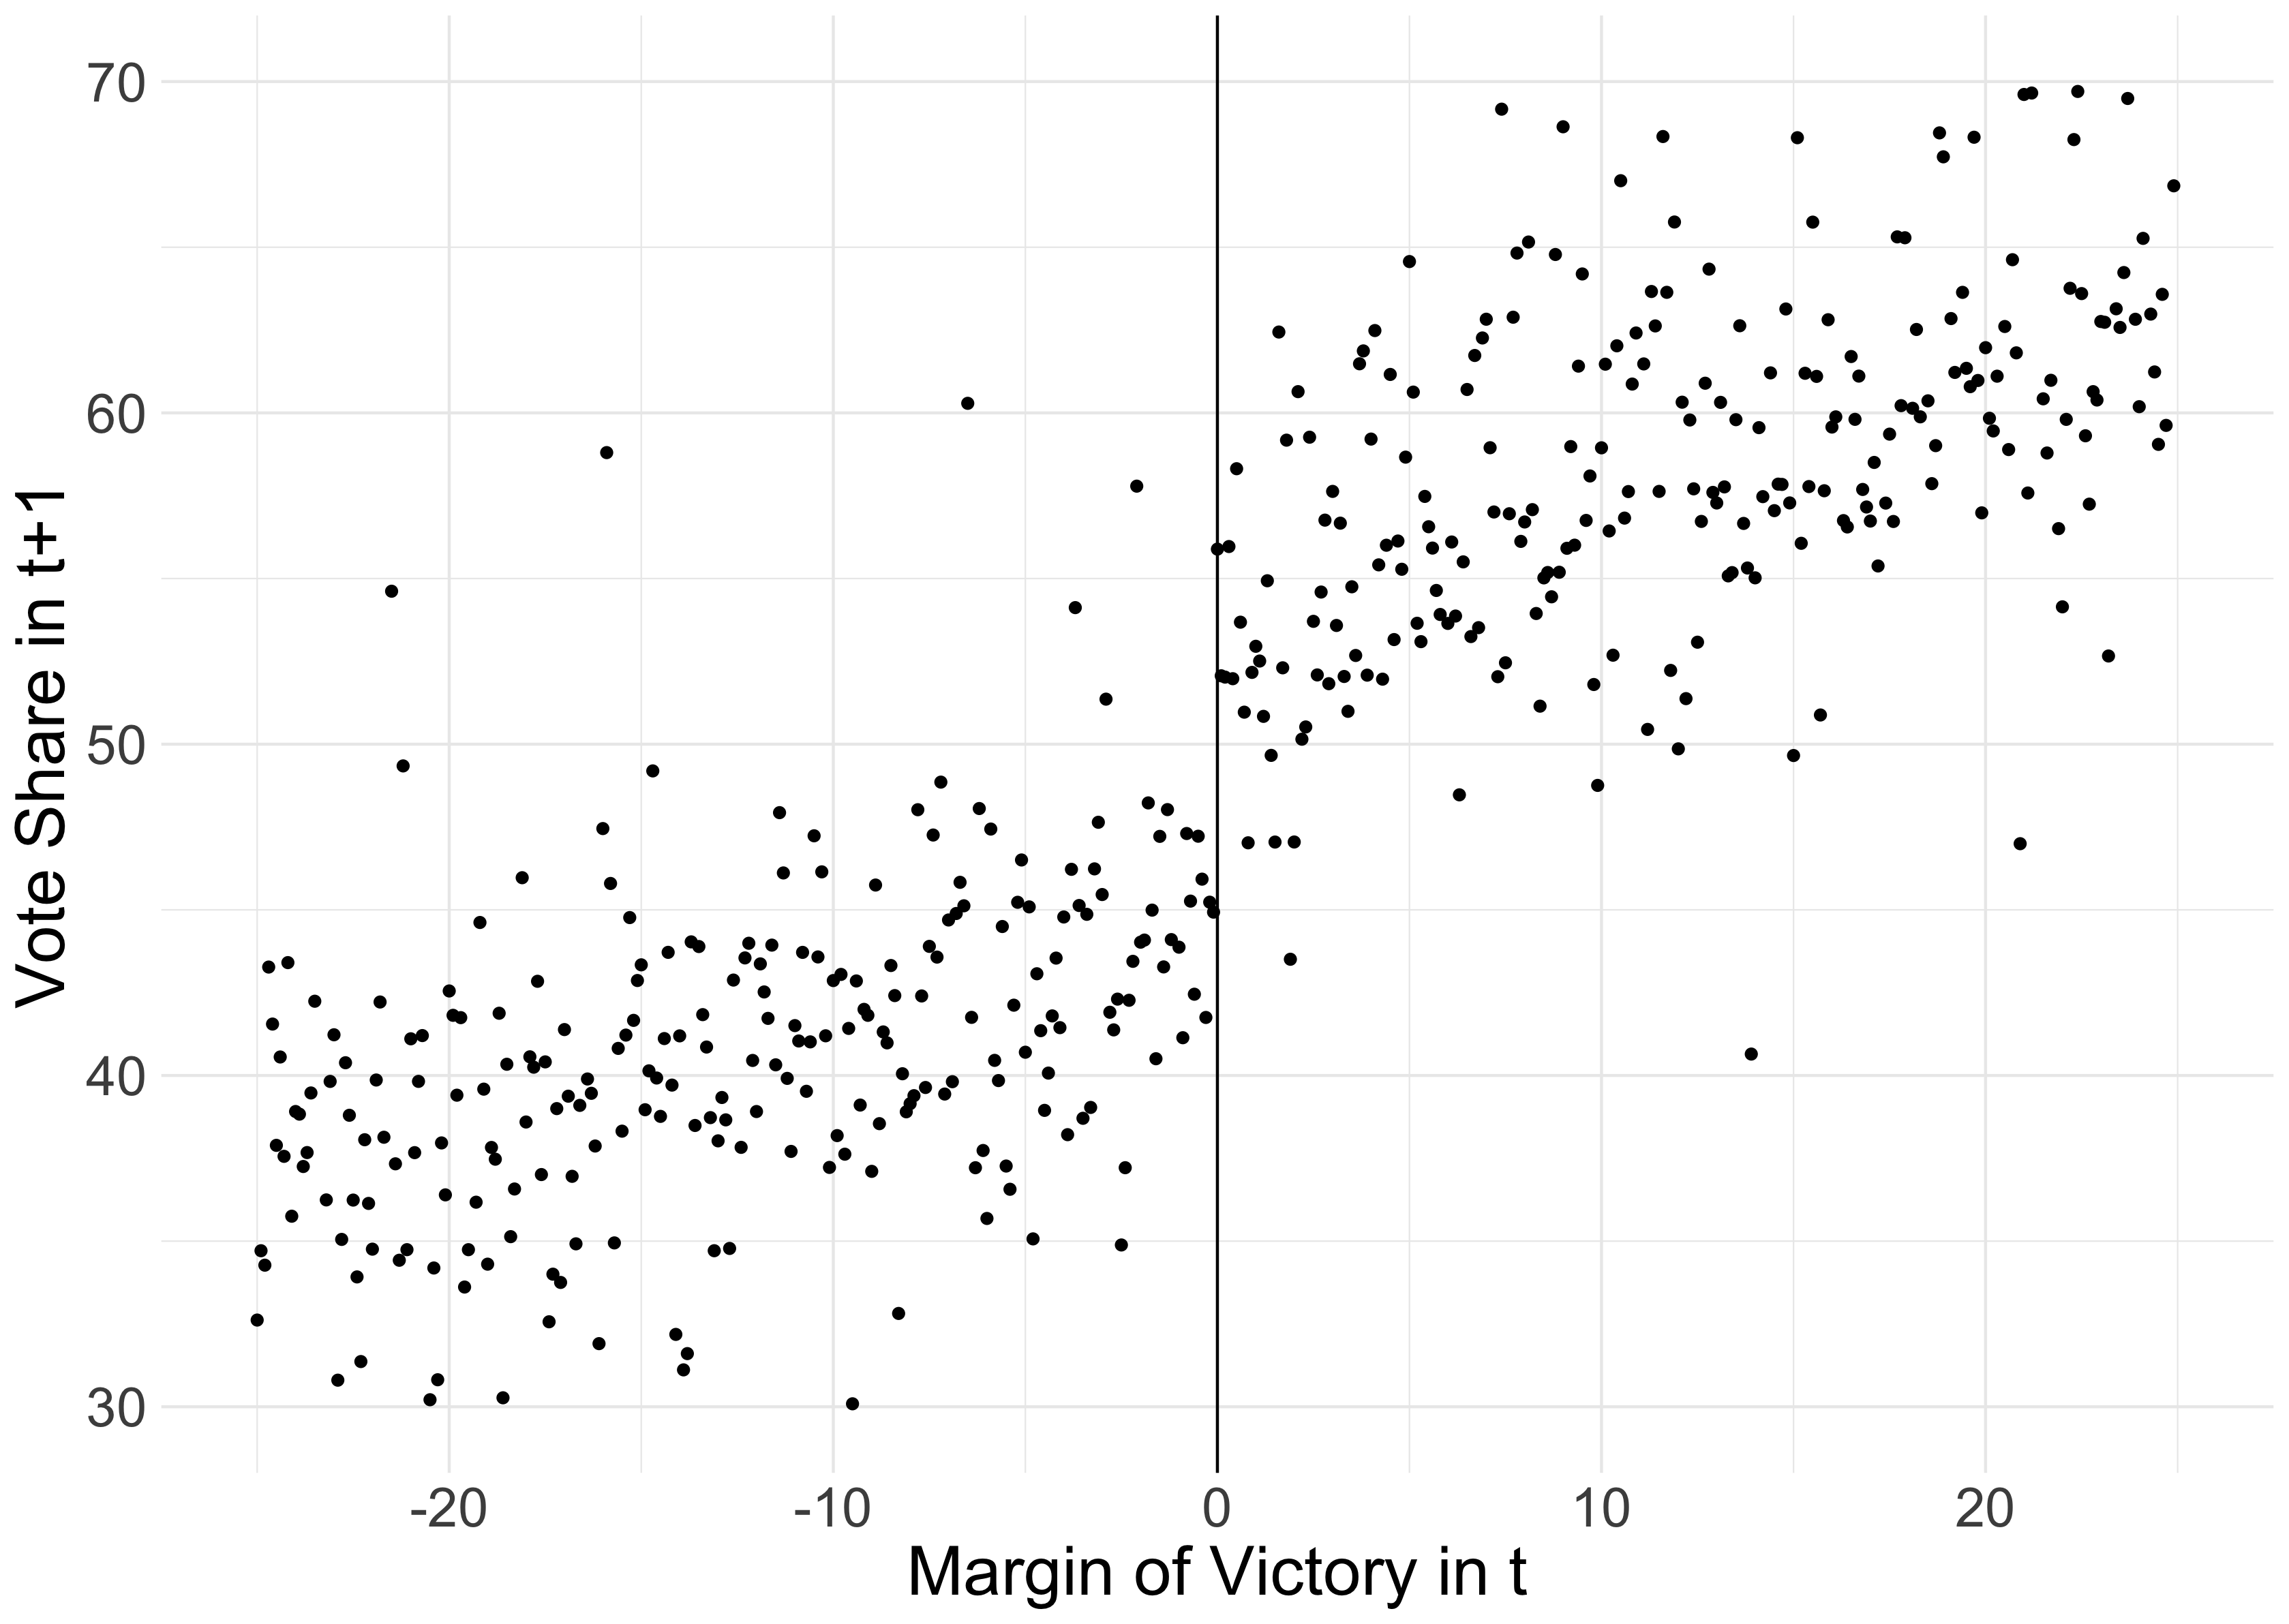
\includegraphics[width=\linewidth]{images/lee_rd_binscatter1e.png}      }
    \end{column}%
  \end{columns}
\end{frame}



\begin{frame}{A quick aside on graphical construction}
  \begin{columns}[onlytextwidth, T] % align columns
    \begin{column}{.5\textwidth}
      \begin{wideitemize}
      \item Given how graphically important bin choice is, how should
        we choose it?
      \item Turns out there are two important decisions:
        \begin{itemize}
        \item How to place the bins: equal-spaced, or quantile
        \item How many bins?
        \end{itemize}
      \item The equal-spaced vs. quantile choice is somewhat
        arbitrary, but quantile binning is more transparent
        \begin{itemize}
        \item Choice of equally spaced bins can mask underlying
          density (not so much in this case)
        \end{itemize}

      \end{wideitemize}
    \end{column}%
    \hfill%
    \begin{column}{.5\textwidth}
      \only<1>{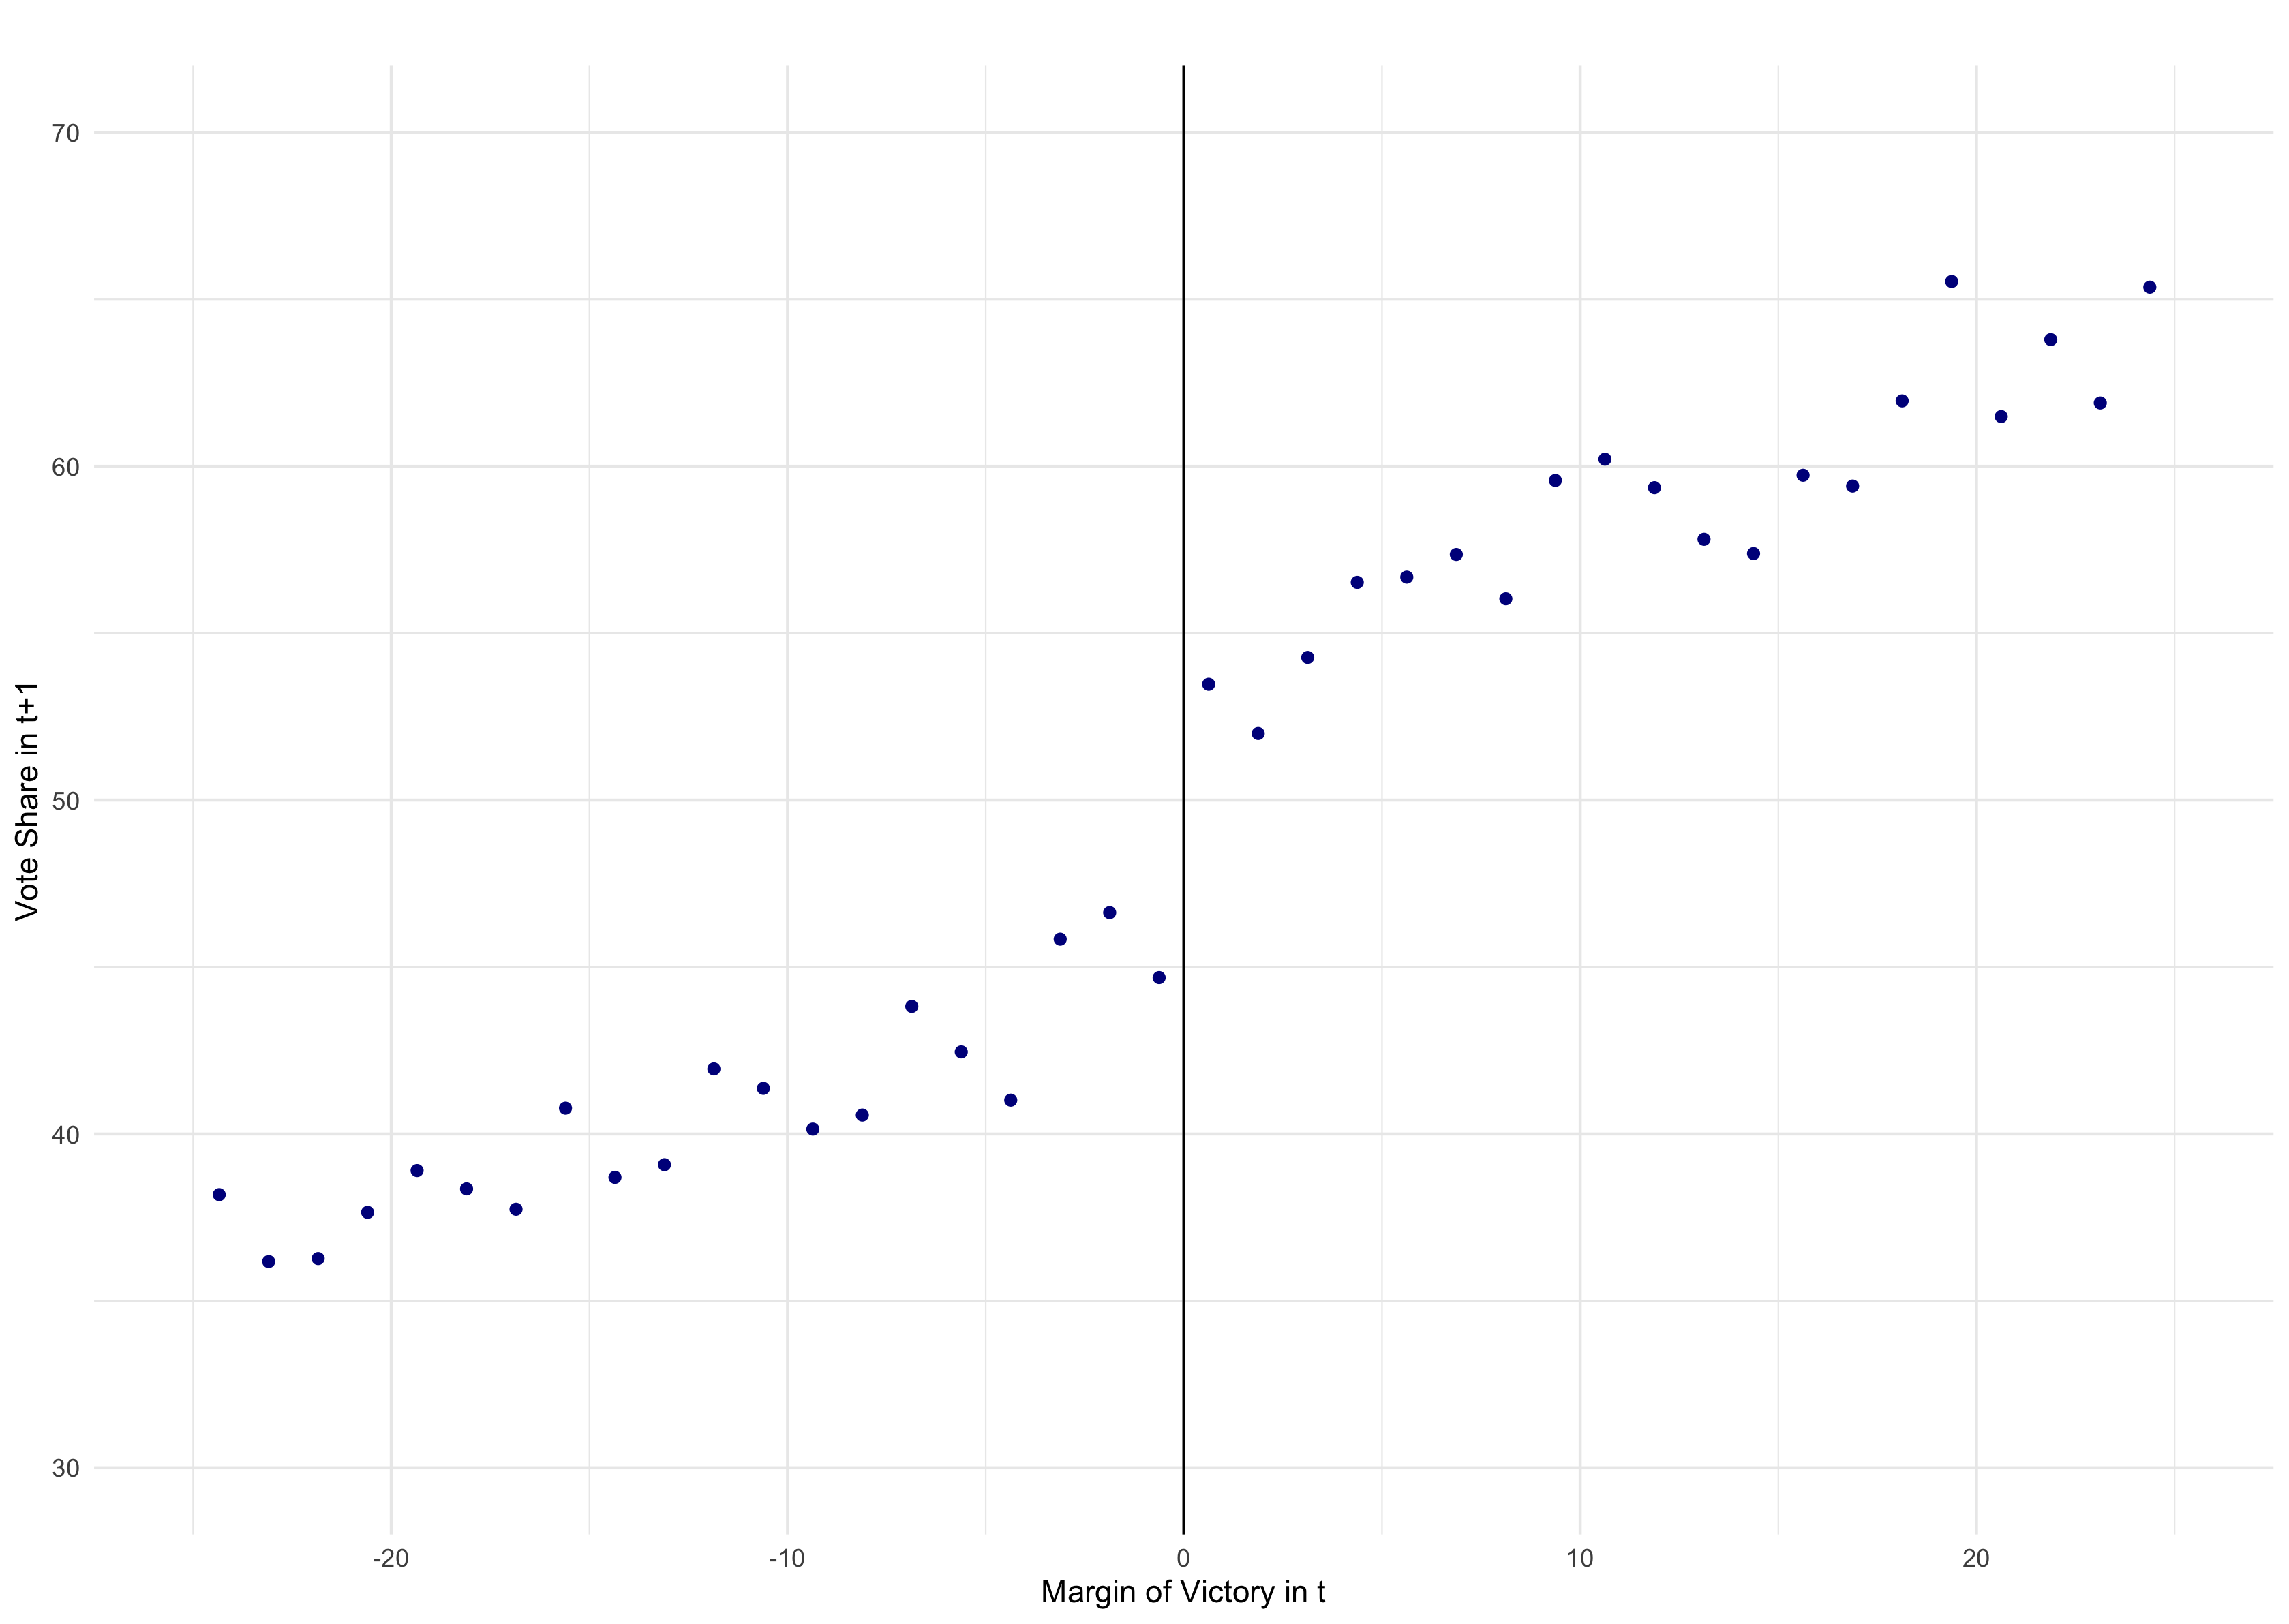
\includegraphics[width=\linewidth]{images/lee_rd_binscatter_es.png}}
      \only<2->{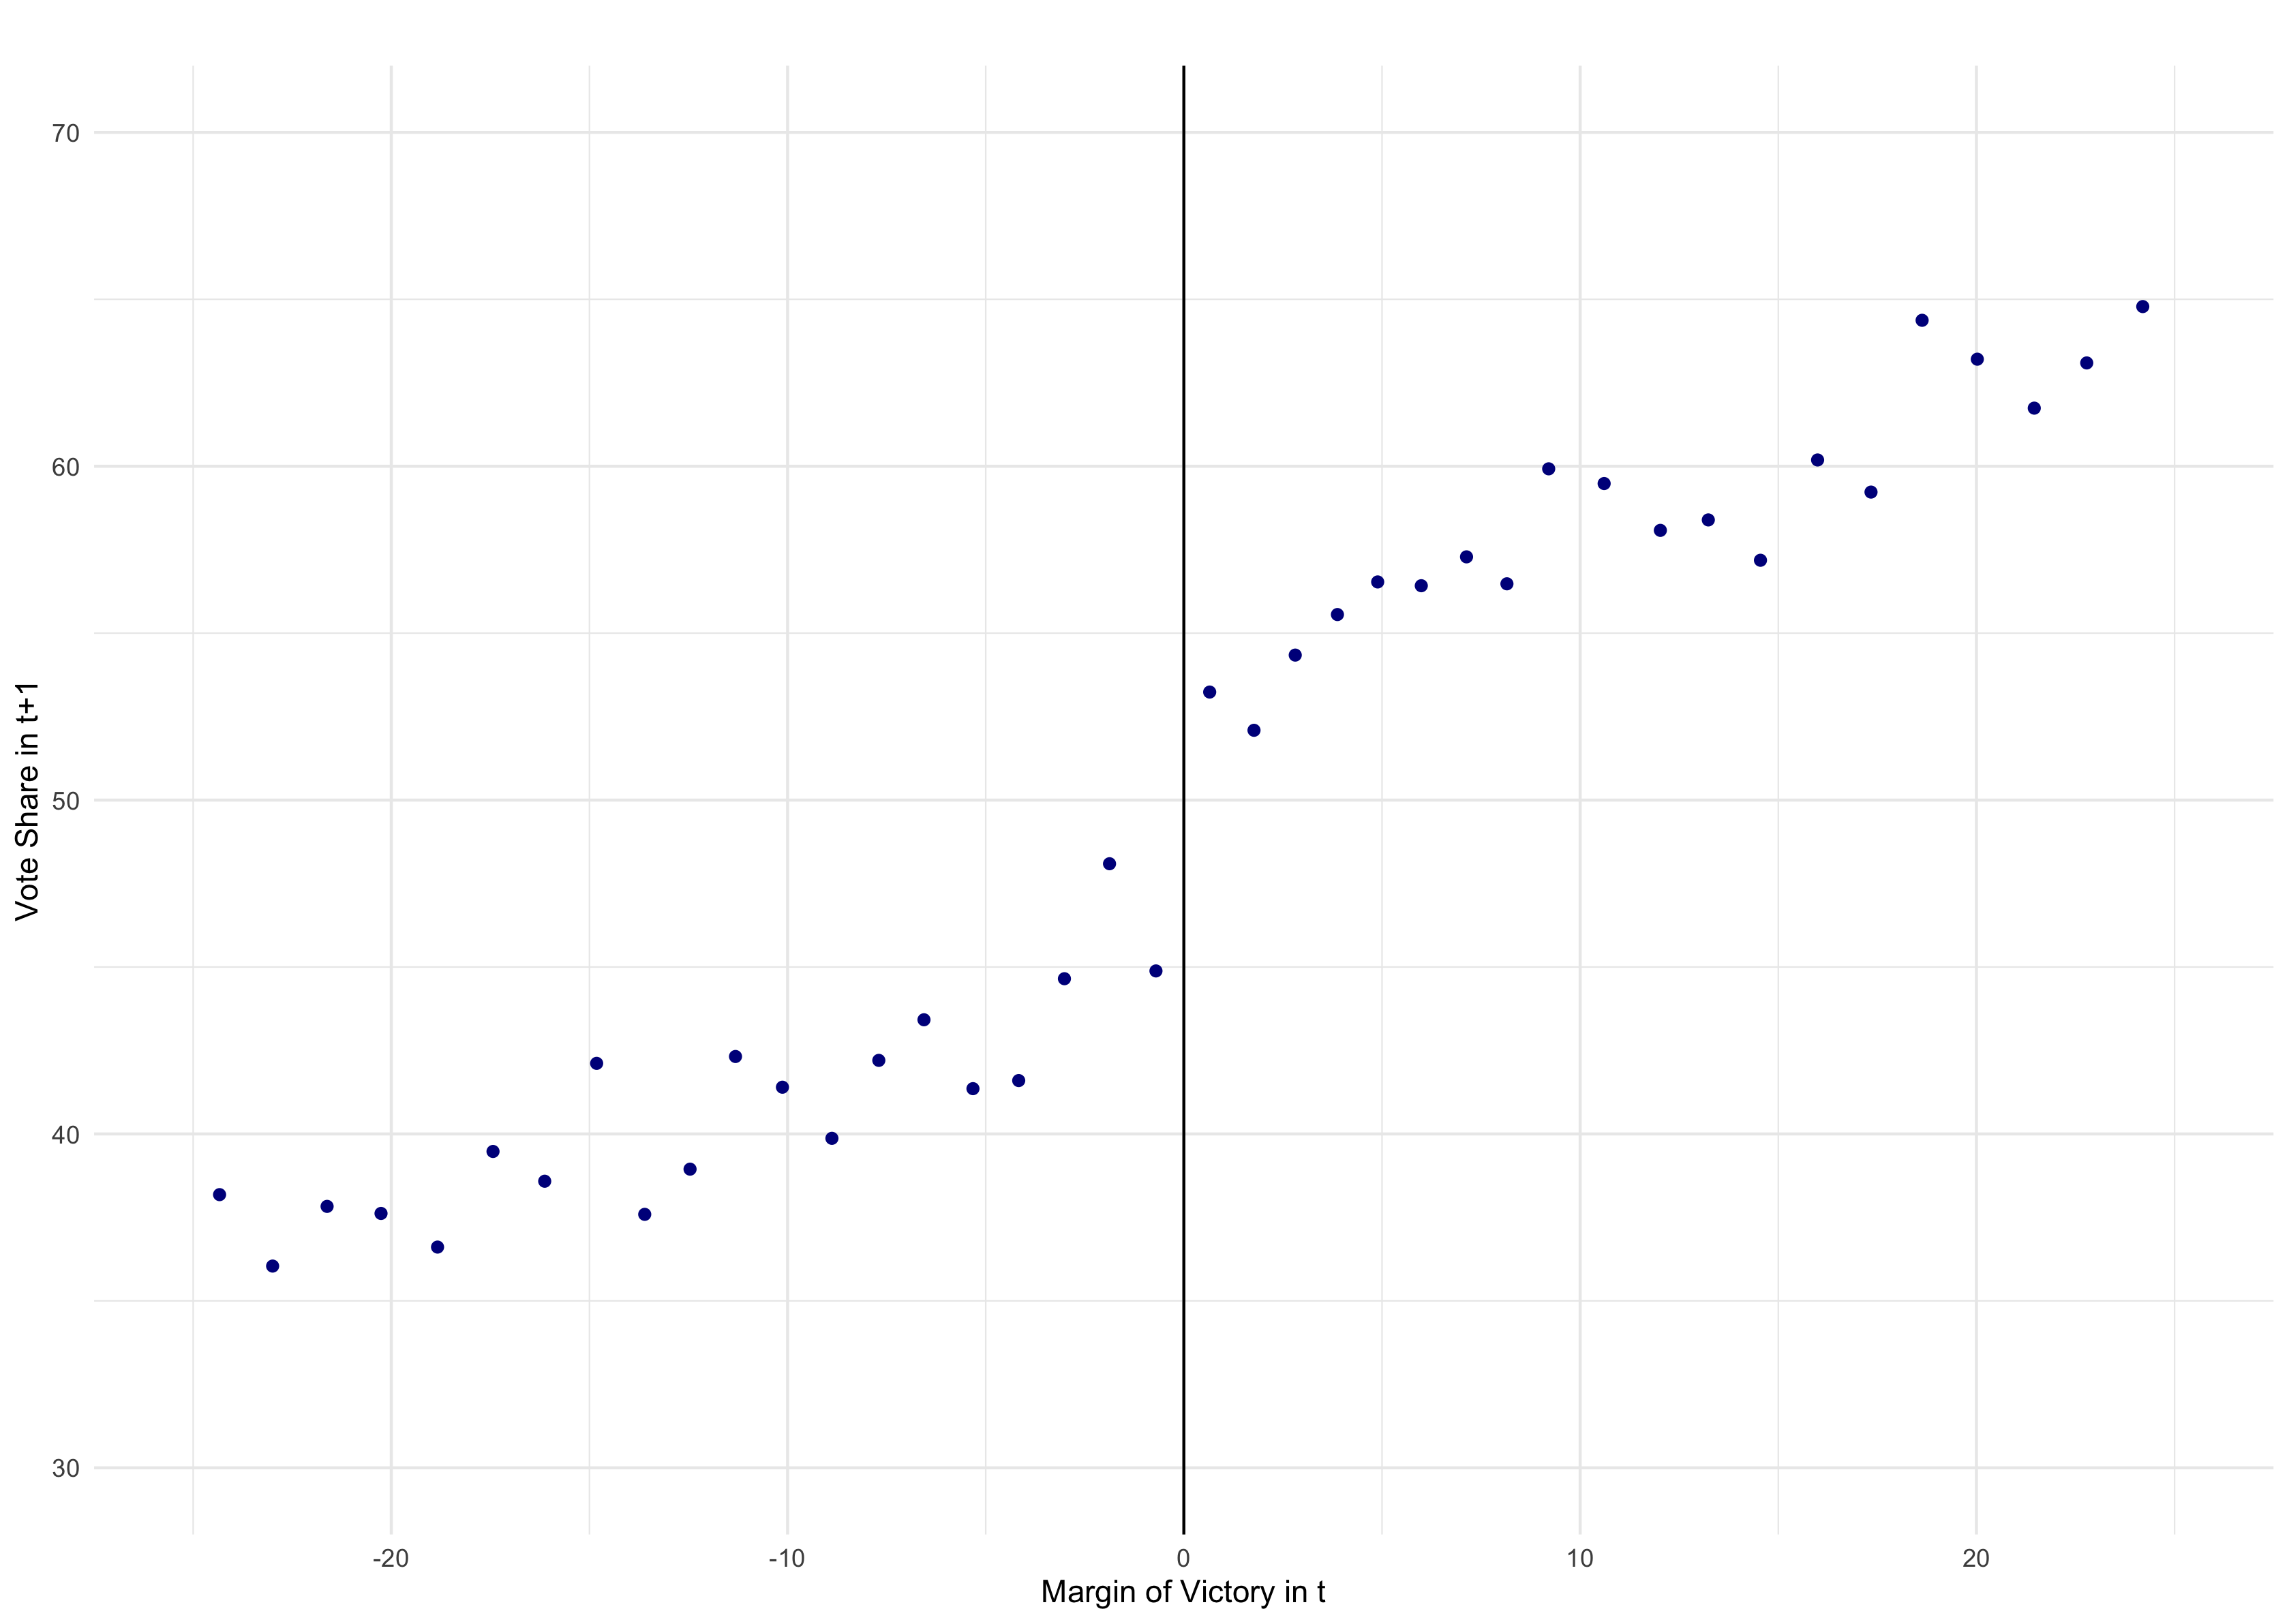
\includegraphics[width=\linewidth]{images/lee_rd_binscatter_qs.png}      }
    \end{column}%
  \end{columns}
\end{frame}

\begin{frame}{A quick aside on graphical construction}
  \begin{columns}[onlytextwidth, T] % align columns
    \begin{column}{.5\textwidth}
      \begin{wideitemize}
      \item Once we choose how to do bins, how should we choose the number?
        \begin{itemize}
        \item Can we choose ``optimally''?
        \end{itemize}
      \item Cattaneo et al. (2020) argue for two approaches (available
        in \texttt{rdrobust}'s \texttt{rdplot}): IMSE-minimizing, and
        mimicking variance.
        \begin{itemize}
        \item IMSE-minimizing trades off between bias and variance in
          choice of bins, but does it over the whole range --
          proportional to $n^{1/3}$
        \item Mimicking-variance tries to match the underlying
          variance of the raw data in the binned plots -- proportional to $n/ \log(n)^{2}$
        \end{itemize}
      \end{wideitemize}
    \end{column}%
    \hfill%
    \begin{column}{.5\textwidth}
      \only<1>{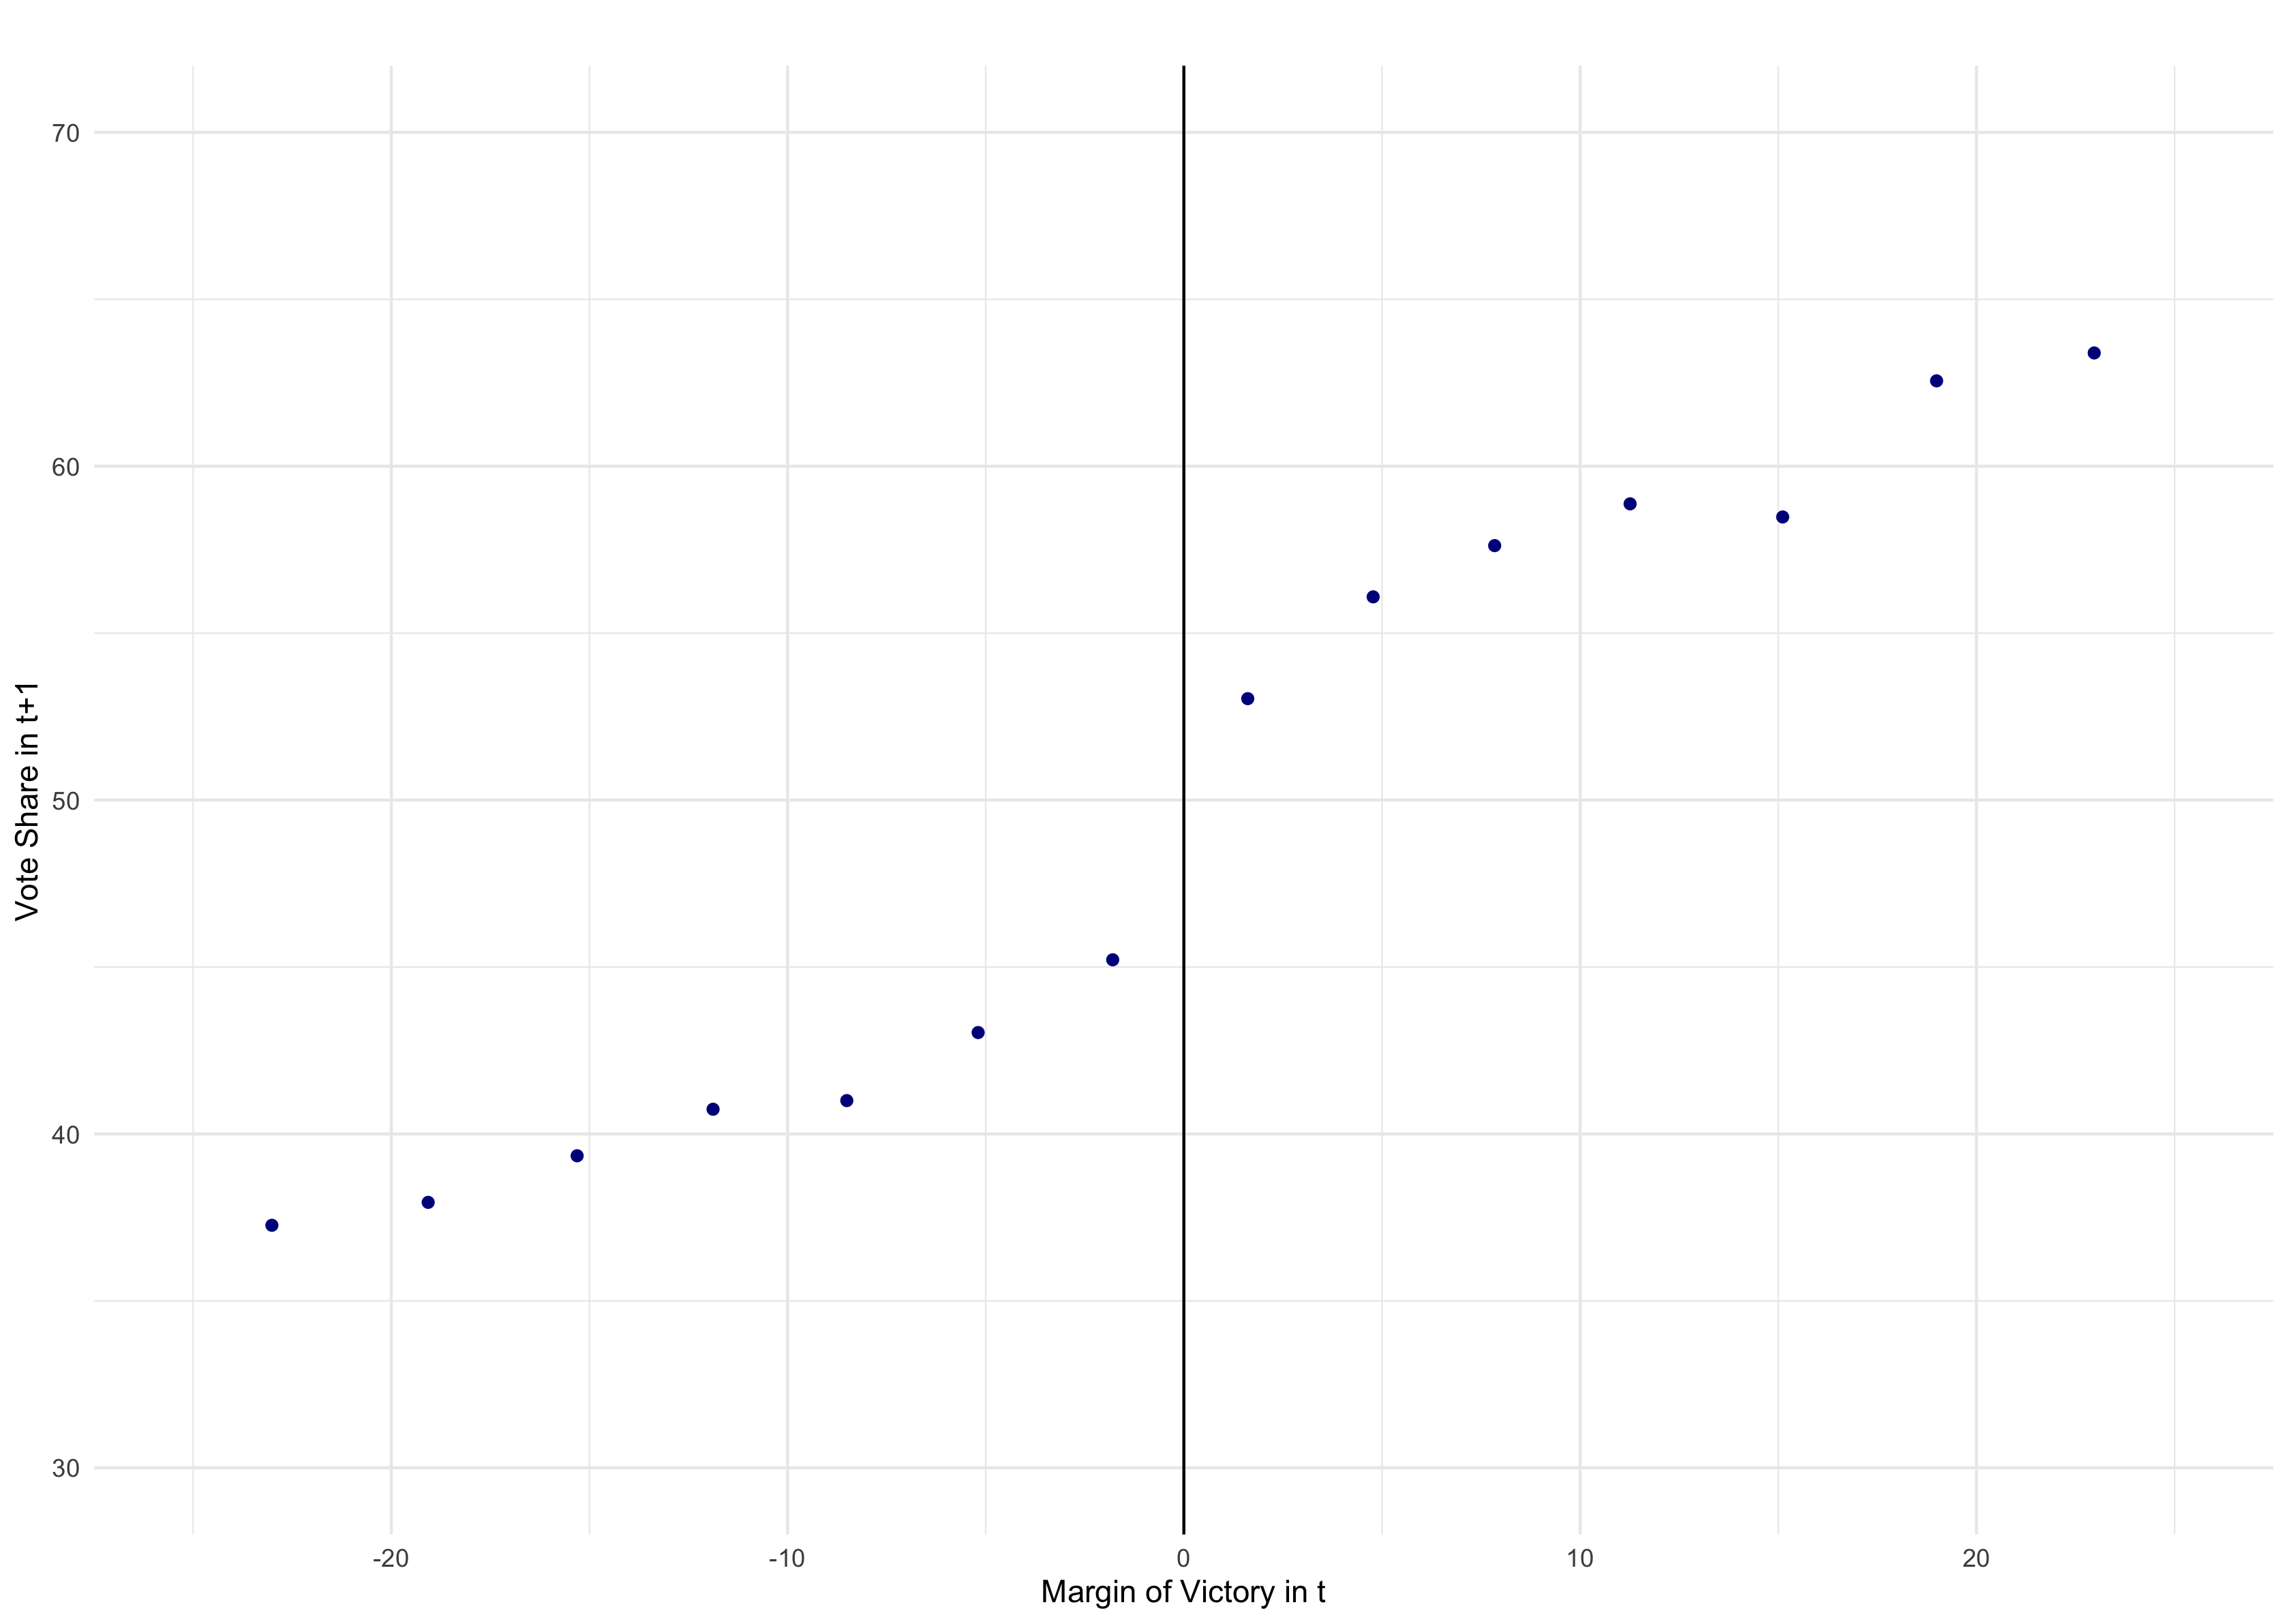
\includegraphics[width=\linewidth]{images/lee_rd_binscatter_qs_choice.png}}
      \only<2->{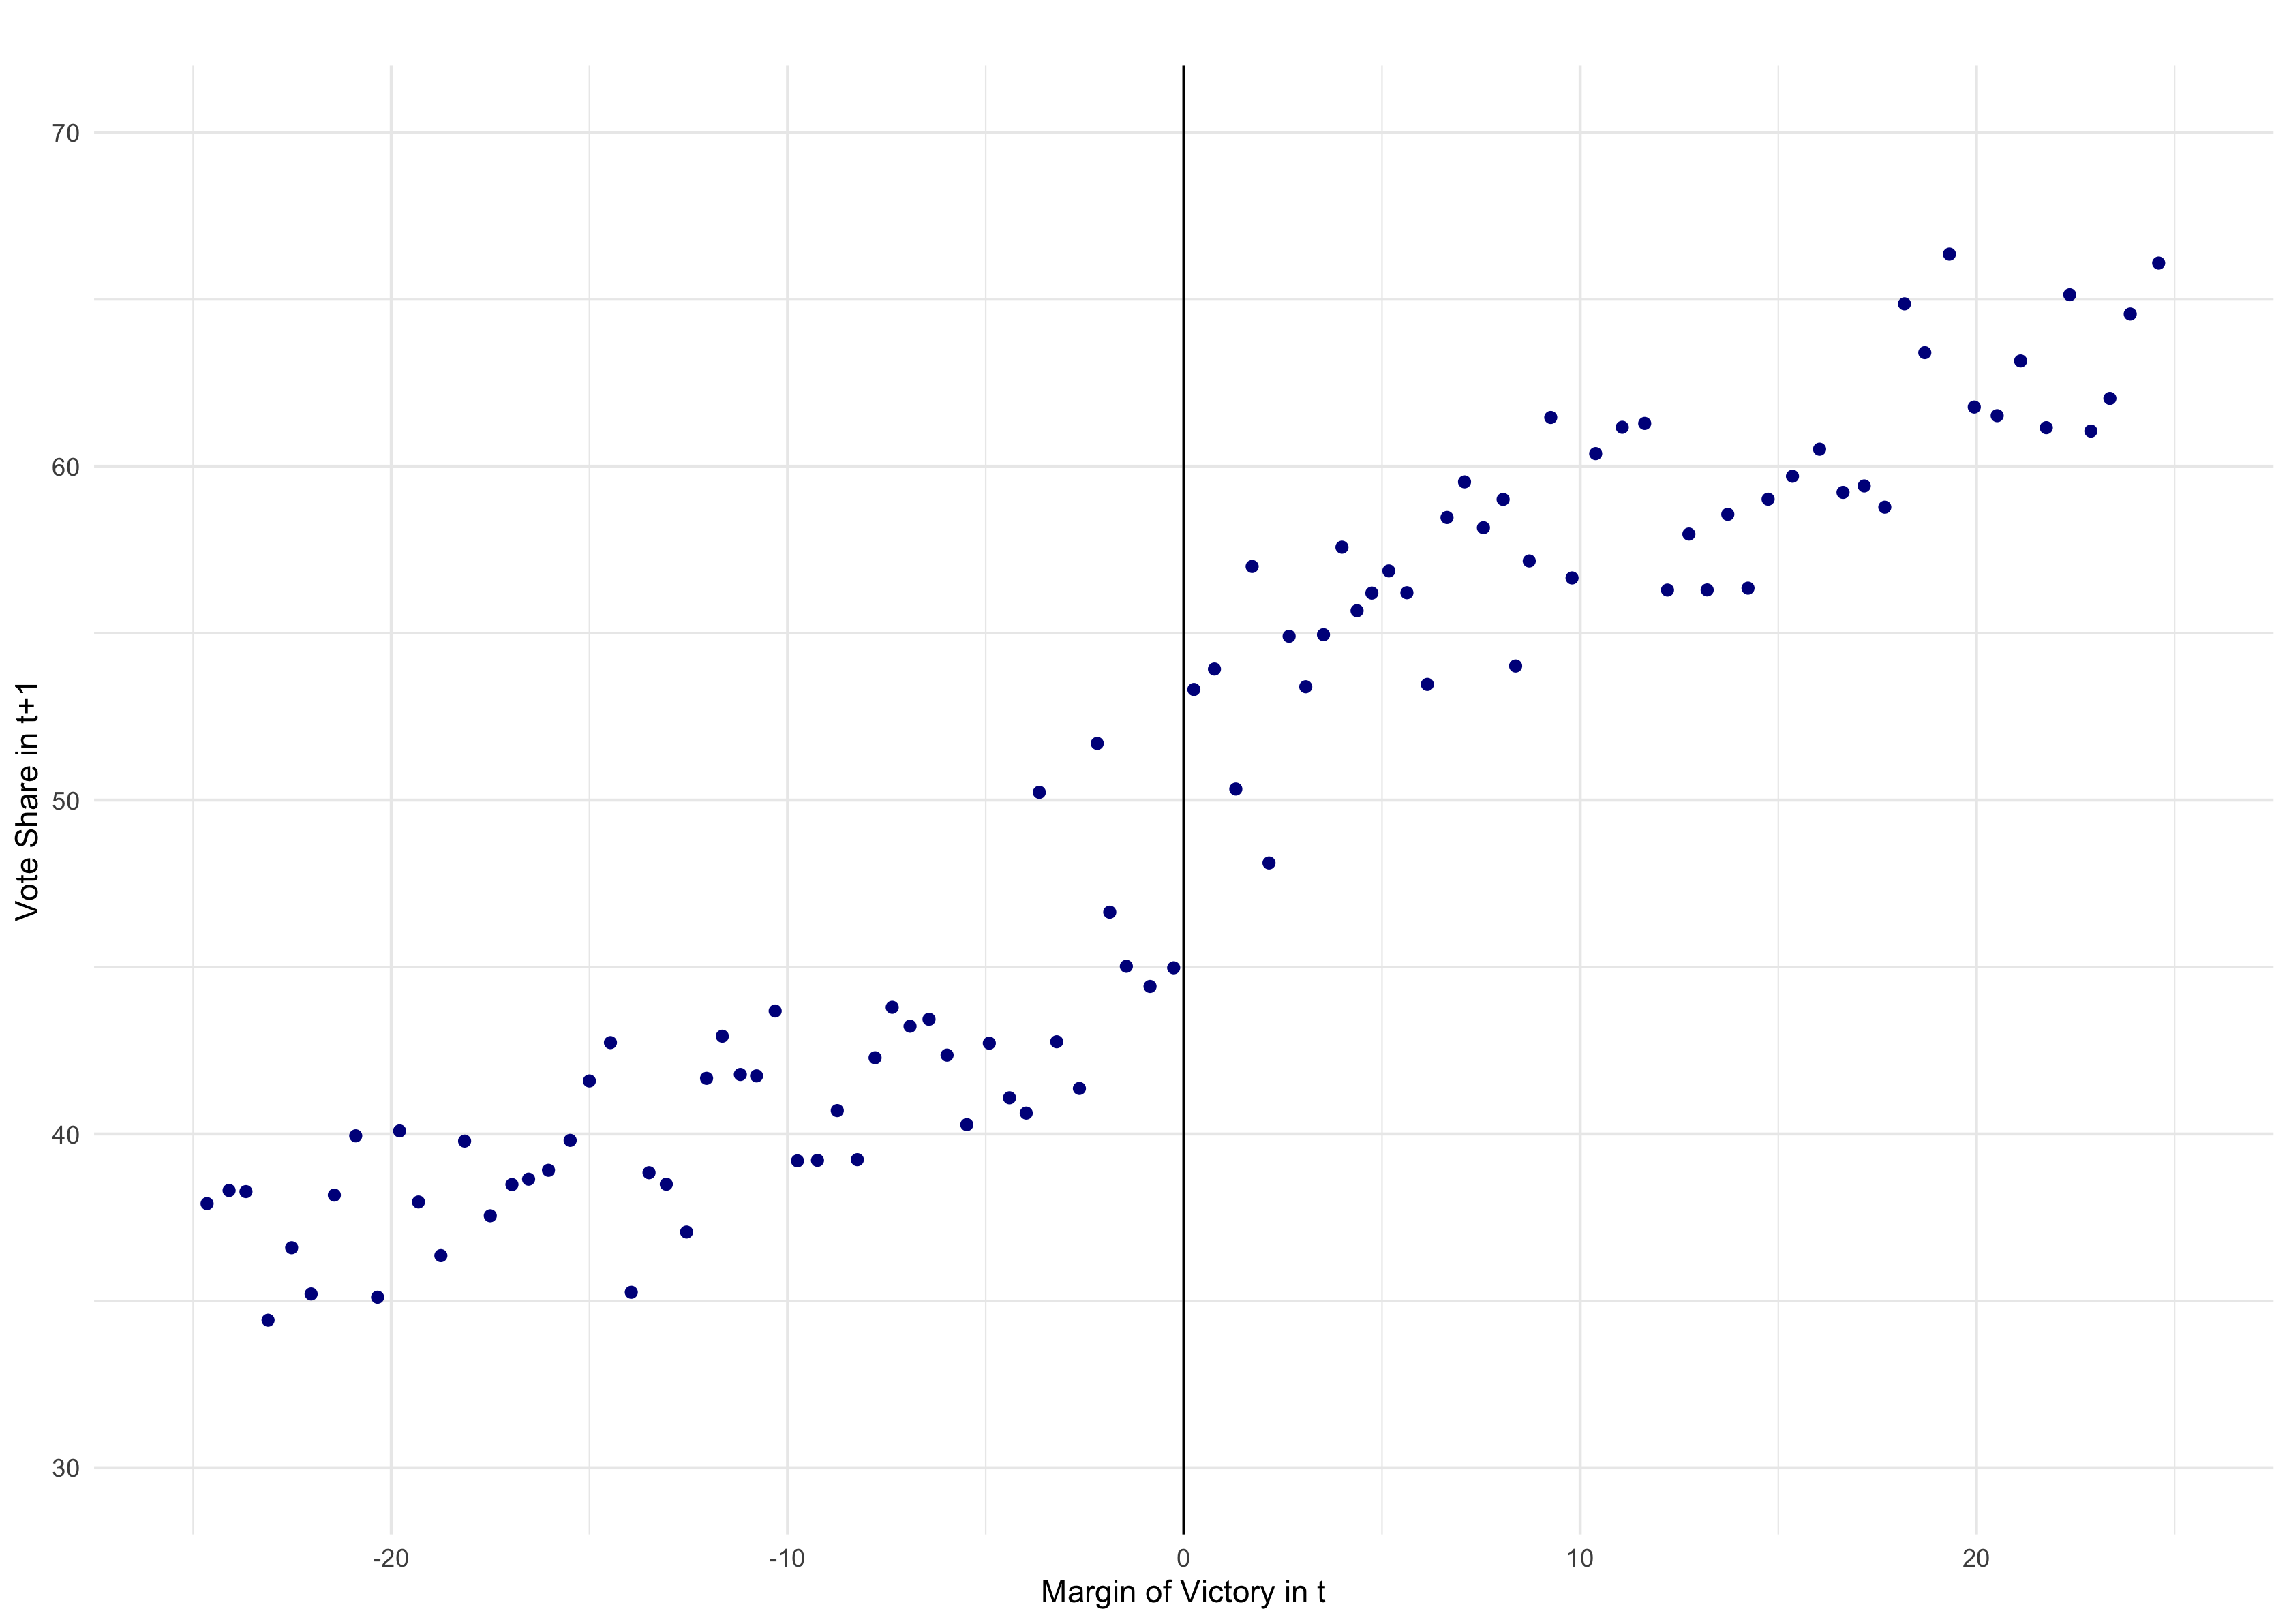
\includegraphics[width=\linewidth]{images/lee_rd_binscatter_qsmv_choice.png}      }
    \end{column}%
  \end{columns}
\end{frame}


\begin{frame}{A quick aside on graphical construction}
  \begin{columns}[onlytextwidth, T] % align columns
    \begin{column}{.5\textwidth}
      \begin{wideitemize}
      \item Obviously in the case of discrete random variables, this
        is not complicated! We would just bin directly on the discrete values
      \item The complicating issues will arise when imputing a smooth
        function on top of these discrete values
      \item See Kolesar and Rothe (2018) for details
      \end{wideitemize}
    \end{column}%
    \hfill%
    \begin{column}{.5\textwidth}
    \end{column}%
  \end{columns}
\end{frame}
\begin{frame}{Checking for balance}
  \begin{columns}[onlytextwidth, T] % align columns
    \begin{column}{\textwidth}
      \begin{wideitemize}
      \item As we discussed above, key test is to compare the averages
        of other variables at $Z = 0$, the cutoff.
      \item Canay and Kamat (2017) show that if you are willing to
        assume a slightly stronger assumption -- e.g. that choice of
        location around the cutoff is not fully deterministic -- then
        you can do better
      \item Key points:
        \begin{itemize}
        \item Testing just mean differences doesn't look at other
          parts of the distribution (which may more obviously violate
          this) and so may have low power
        \item B/c the local sample size is effectively small, this can
          create problematic inference issues if the function is not
          particular smooth
        \end{itemize}
      \item They propose a permutation test, which has better
        statistical properties
        \begin{itemize}
        \item Key intuition -- covariates should be
          \emph{approximately} identically distributed on each side of
          the cutoff
        \item This is an \emph{asymptotic} argument, since it's not
          actually a random experiment!
        \end{itemize}
      \end{wideitemize}
    \end{column}%
    \hfill%
    \begin{column}{.5\textwidth}
    \end{column}%
  \end{columns}
\end{frame}

\begin{frame}{Checking for balance- Canay and Kamat}
  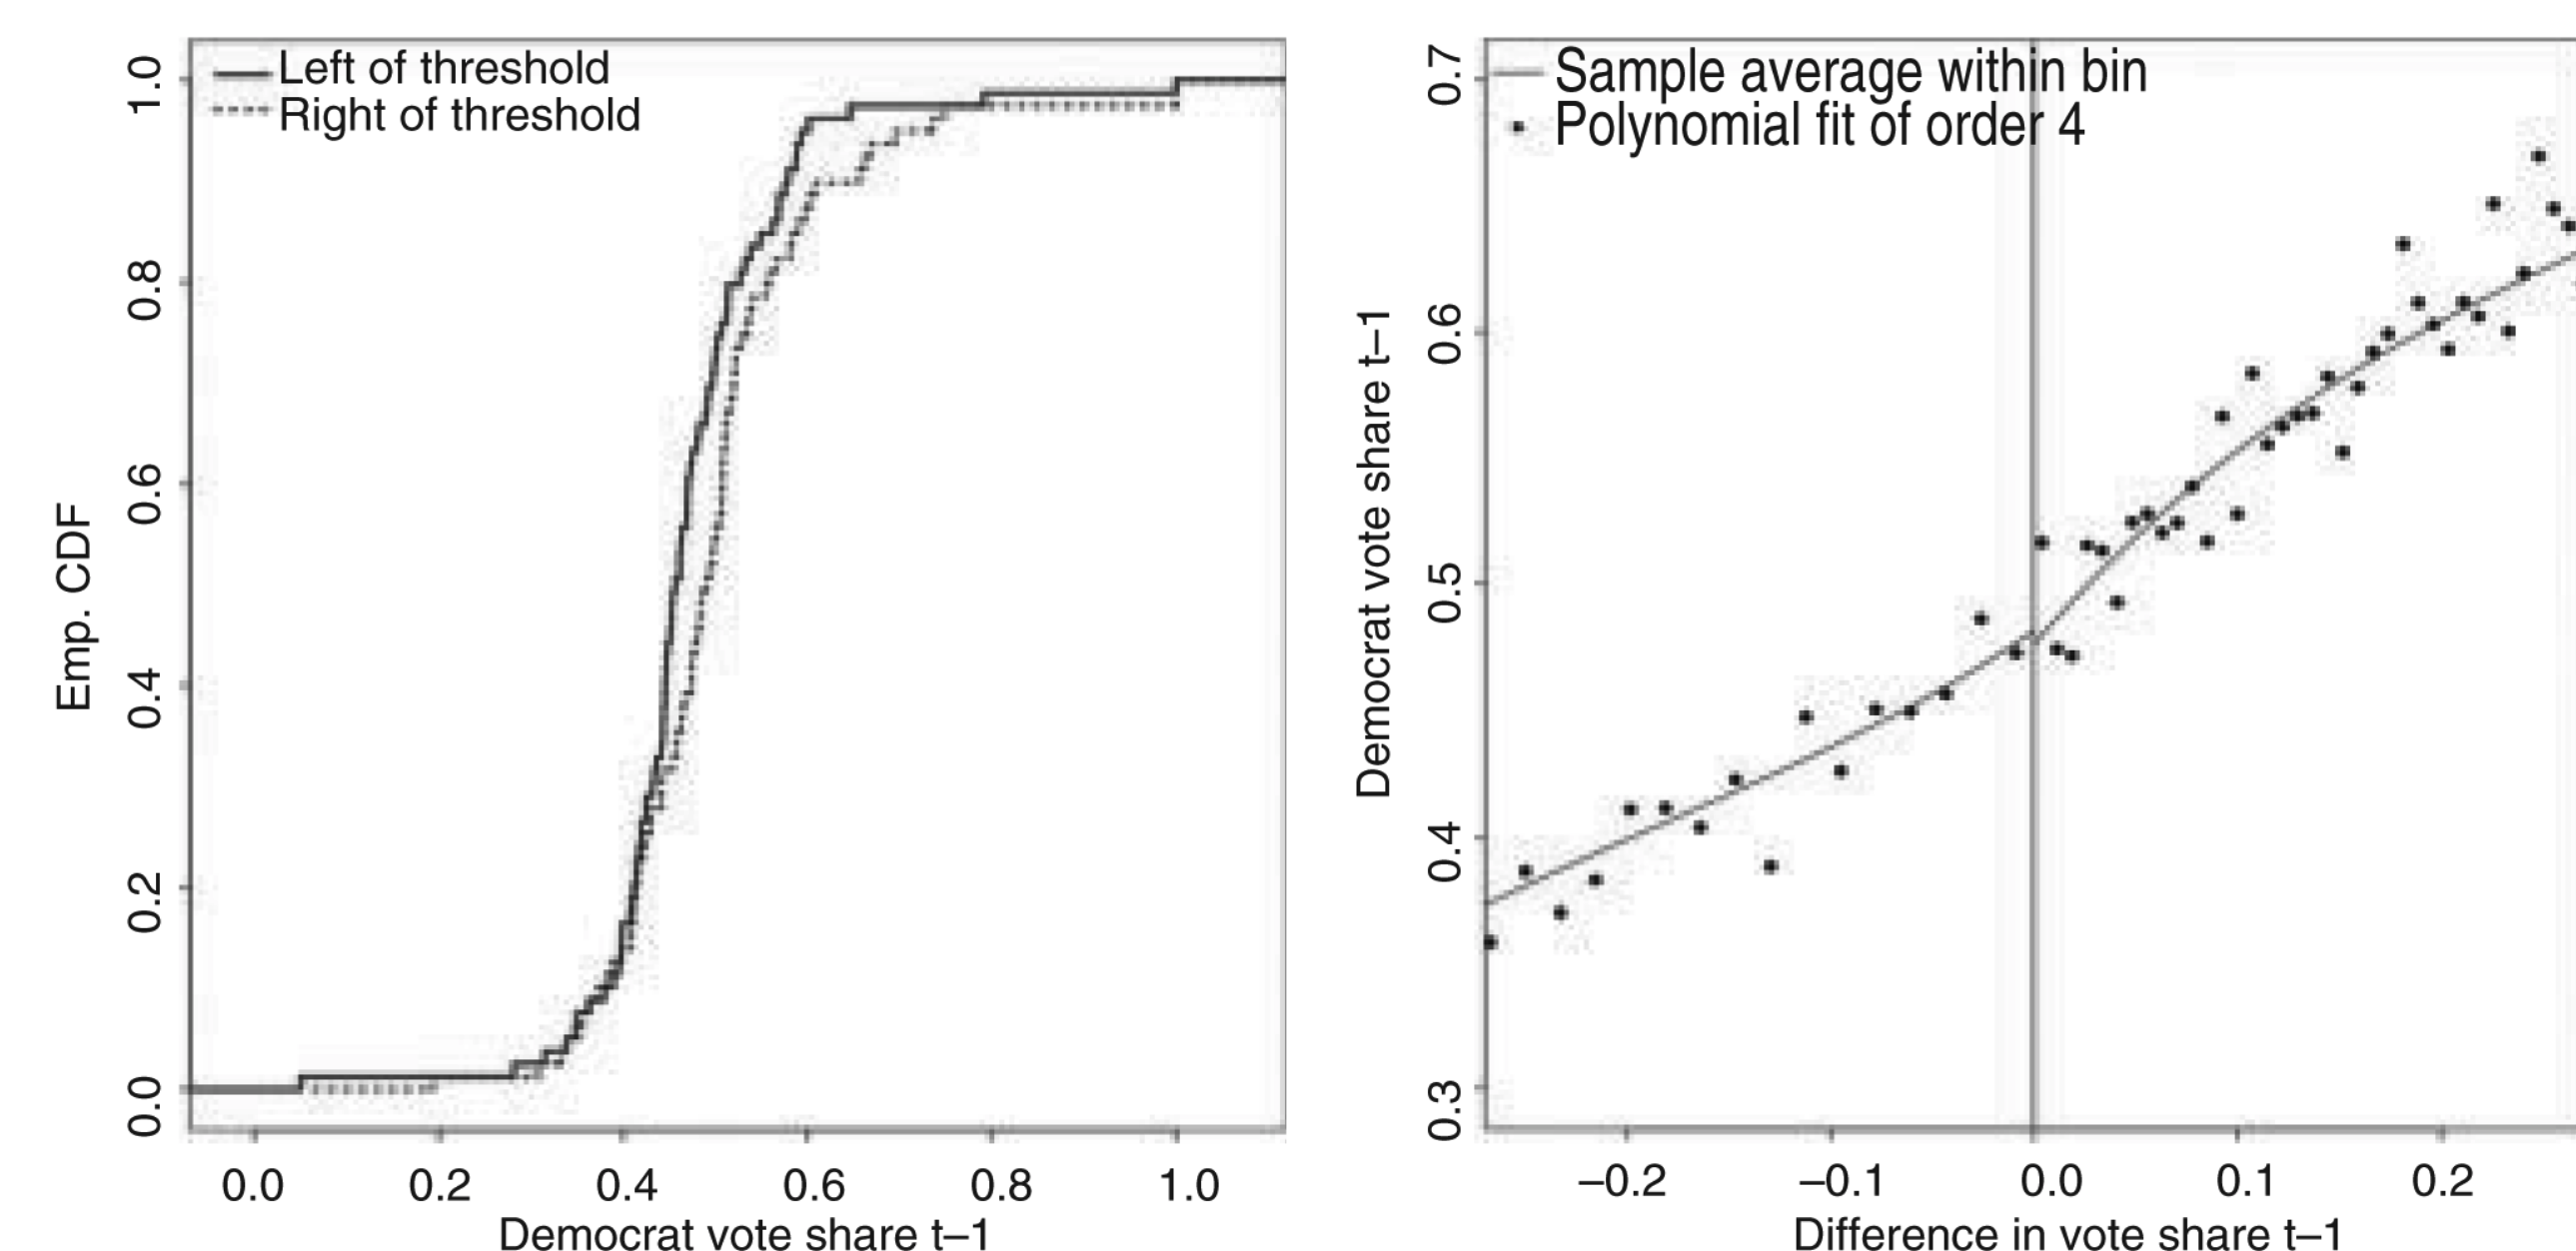
\includegraphics[width=\linewidth]{images/lee_rd_canay.png}
\end{frame}

\begin{frame}{Checking for balance- Canay and Kamat}
  \begin{wideitemize}
  \item This approach requires a slightly stronger assumption than the
    necessary assumptions for identification
  \item E.g., this paper riffs off of Lee (2008) assumption that units
    are effectively permuted around the cutoff (somewhat randomly),
    such that the covariate distribution should be continuous at the
    cutoff
  \item Code is available in Stata and R: \texttt{rdperm} and
    \texttt{RATest}
  \end{wideitemize}
\end{frame}




\begin{frame}{Testing for bunching in forcing variable}
    \begin{columns}[onlytextwidth, T] % align columns
      \begin{column}{.5\textwidth}
        \begin{wideitemize}
        \item Similar to the balance test, Mcrary (2008) proposed a
          test of the continuitiy in the density of the running
          variable
        \item In essence, is there ``bunching'' in the characteristic
          on one side or the other?
          \begin{itemize}
          \item This intuition makes sense economically -- if there's
            a benefit of being on one side, why would you not
            ``shift'' yourself across the boundary?
          \end{itemize}
        \item This is easily tested by comparing the values of an
          estimated density on the left and right of the cutoff
        \item Software is also available for this! \texttt{rddensity}
          in Stata and R
        \end{wideitemize}
      \end{column}%
      \hfill%
      \begin{column}{.5\textwidth}
      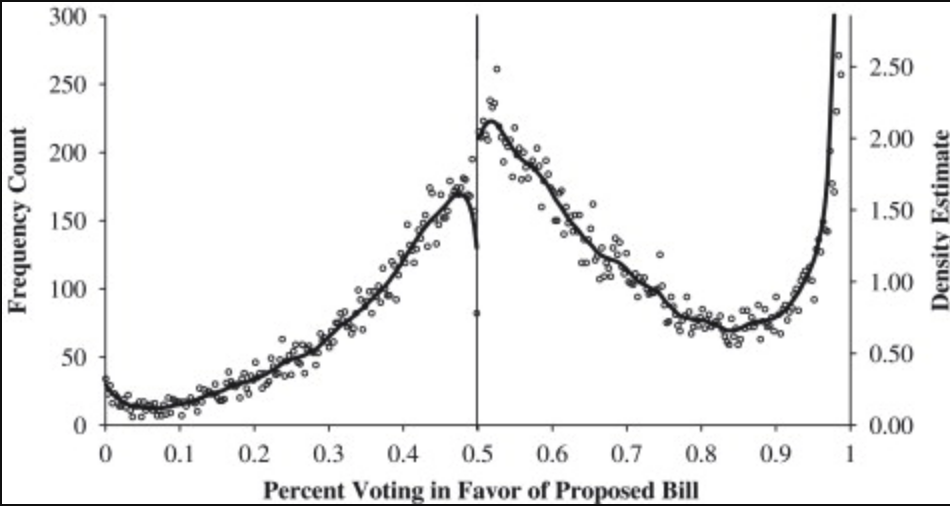
\includegraphics[width=\linewidth]{images/mcrary_1.png}
      \end{column}%
    \end{columns}
\end{frame}

\begin{frame}{Testing for bunching in forcing variable}
    \begin{columns}[onlytextwidth, T] % align columns
      \begin{column}{0.7\textwidth}
        \begin{wideitemize}
        \item Placebo checks are less formalized (or at least I know them less well)
        \item Ganong and Jager (2017) propose permutation tests for
          randomizing the location of the cutoff
          \begin{itemize}
          \item This method presumably works as well in the RD setting 
          \end{itemize}
        \item Intuitively, one would pick cutoffs above and below the
          true cutoff, and test for jumps in the outcome. If these are
          insignificant, that gives credibility to the design
          \begin{itemize}
          \item More formally, using a permutation test, one could
            permute the cutoff and look at the relative effect of the
            true effect compared to the null distribution
          \item Effectively treats the choice of cutoff as the random
            design variable
          \end{itemize}
        \end{wideitemize}
      \end{column}%
      \hfill%
      \begin{column}{.5\textwidth}
      \end{column}%
    \end{columns}
\end{frame}

\begin{frame}{Showing our outcome}
    \begin{columns}[onlytextwidth, T] % align columns
      \begin{column}{0.5\textwidth}
        \begin{wideitemize}
        \item Finally, we plot our outcome.
        \item This involves both a plotting of the binned data, as
          well as our choice of the conditional mean function
        \item Notably, while we plot a large window around the cutoff, the window of plotted points is irrelevant for estimation
          \begin{itemize}
          \item The choice of bandwidth will be smaller than the window 
          \end{itemize}
        \item This is really for the ``eyeball test'' (Korting et al. (2020))
          \begin{itemize}
          \item A good graph is worth a lot! If you have a bad graph... maybe you have a bad experiment?
          \end{itemize}
        \end{wideitemize}
      \end{column}%
      \hfill%
      \begin{column}{.5\textwidth}
        \only<1>{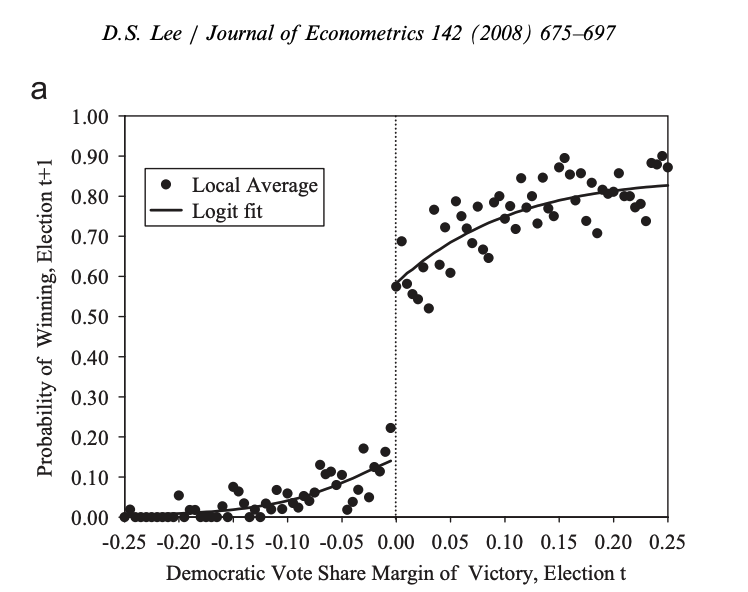
\includegraphics[width=\linewidth]{images/lee_1a.png}}        
      \end{column}%
    \end{columns}
\end{frame}


\begin{frame}{Estimating our outcomes}
    \begin{columns}[onlytextwidth, T] % align columns
      \begin{column}{.7\textwidth}
        \begin{wideitemize}
        \item The actual estimation, as you've seen, is subject to many tuning parameters:
          \begin{itemize}
          \item Choice of estimation procedure, bandwidth, kernel 
          \end{itemize}
        \item Much of this is more automated now, but there is still discretion
        \item My suggestion: use defaults unless you have a very good reason not to
          \begin{itemize}
          \item Defaults: local linear regression, optimized bandwidth
            from estimation procedures in packages (e.g. Cattaneo et
            al.'s \texttt{rdrobust} or Kolesar and Rothe's
            \texttt{RDRobust}), uniform kernel
          \item Even in these categories, there is discretion, but
            important to be consistent and transparent
            \begin{itemize}
            \item See Armstrong and Kolesar (2018) on bandwidth snooping
            \end{itemize}
          \end{itemize}
        \end{wideitemize}
      \end{column}%
      \hfill%
      \begin{column}{.3\textwidth}
      \end{column}%
    \end{columns}
\end{frame}

\begin{frame}{Estimating our outcomes}
    \begin{columns}[onlytextwidth, T] % align columns
      \begin{column}{.5\textwidth}
        \begin{wideitemize}
        \item Also, you can put your estimates directly in the graph! Why waste time with tables
        \end{wideitemize}
      \end{column}%
      \hfill%
      \begin{column}{.5\textwidth}
        \only<1>{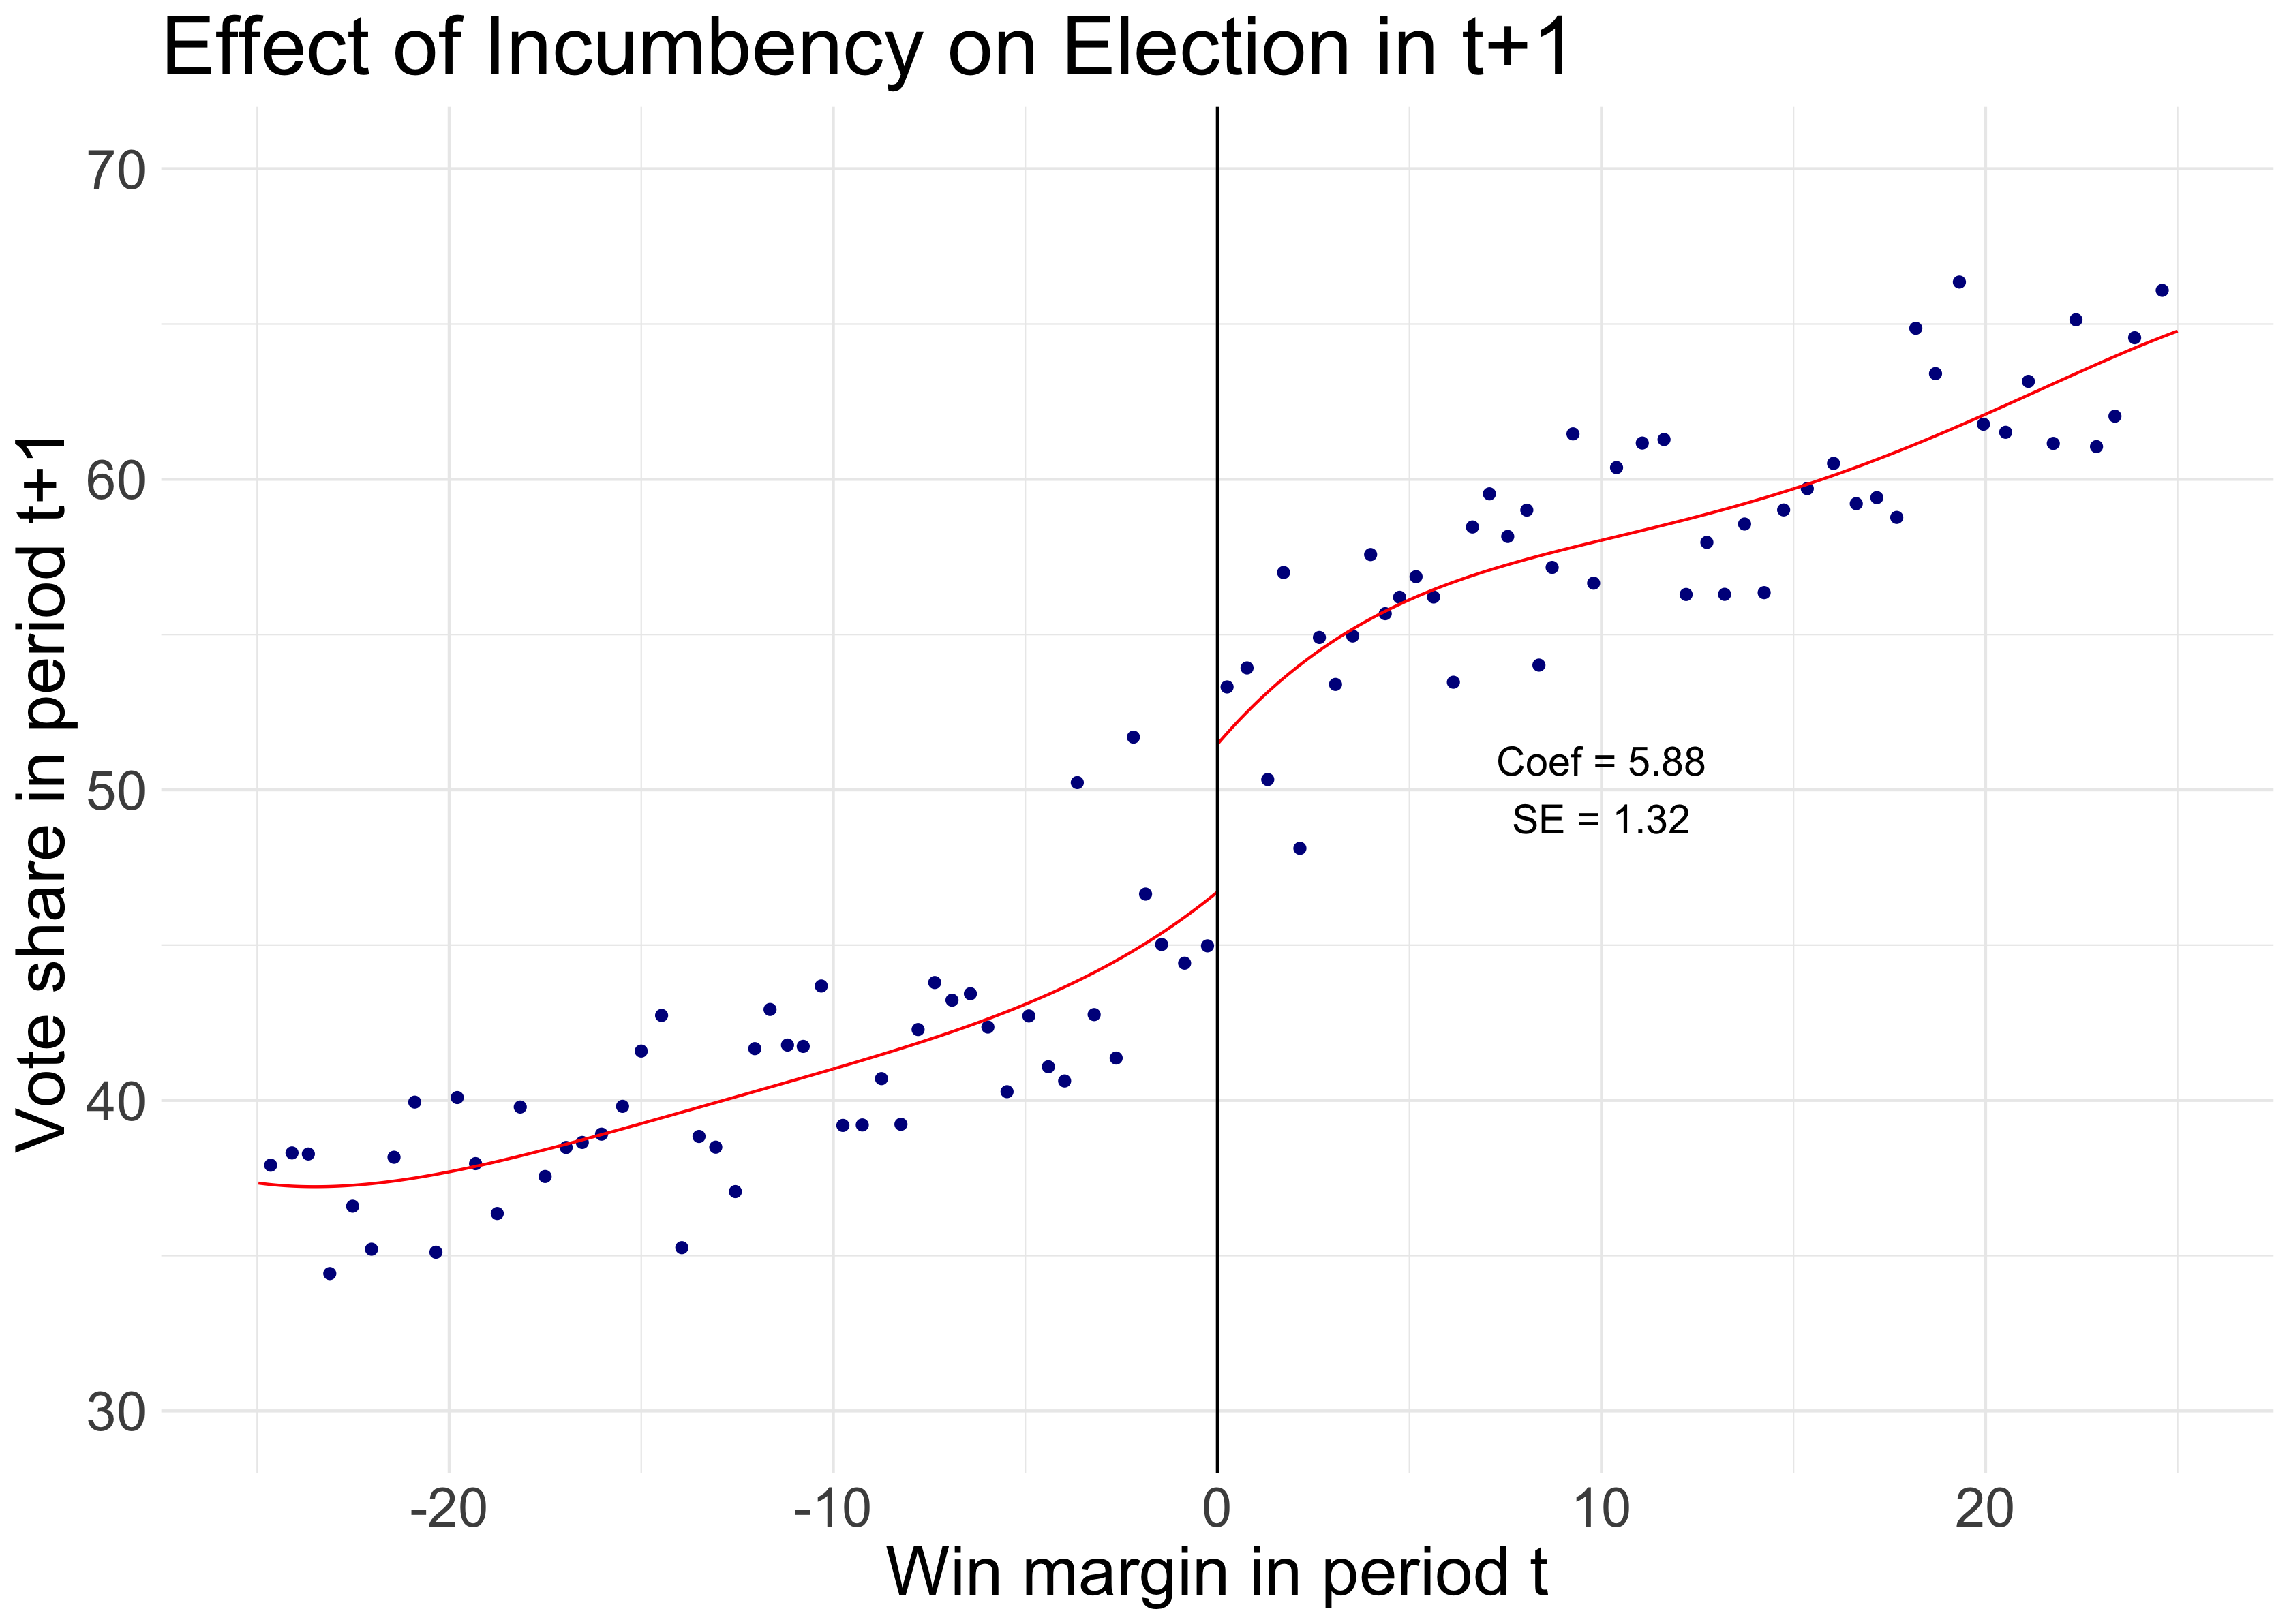
\includegraphics[width=\linewidth]{images/lee_rd_binscatter_output.png}}                
      \end{column}%
    \end{columns}
\end{frame}



\begin{frame}{Showing robustness}
    \begin{columns}[onlytextwidth, T] % align columns
      \begin{column}{.5\textwidth}
        \begin{wideitemize}
        \item Showing robustness is sometimes the only way to convince
          a reader or audience member
          \begin{itemize}
          \item E.g. ``I did this the optimal way!'' is not a good excuse
          \end{itemize}
        \item A simple and clean ways to present your robustness result
          \begin{itemize}
          \item Consider many bandwidths / permutations, and plot how sensitive the estimates are            
          \end{itemize}
        \end{wideitemize}
      \end{column}%
      \hfill%
      \begin{column}{.5\textwidth}
        \only<1>{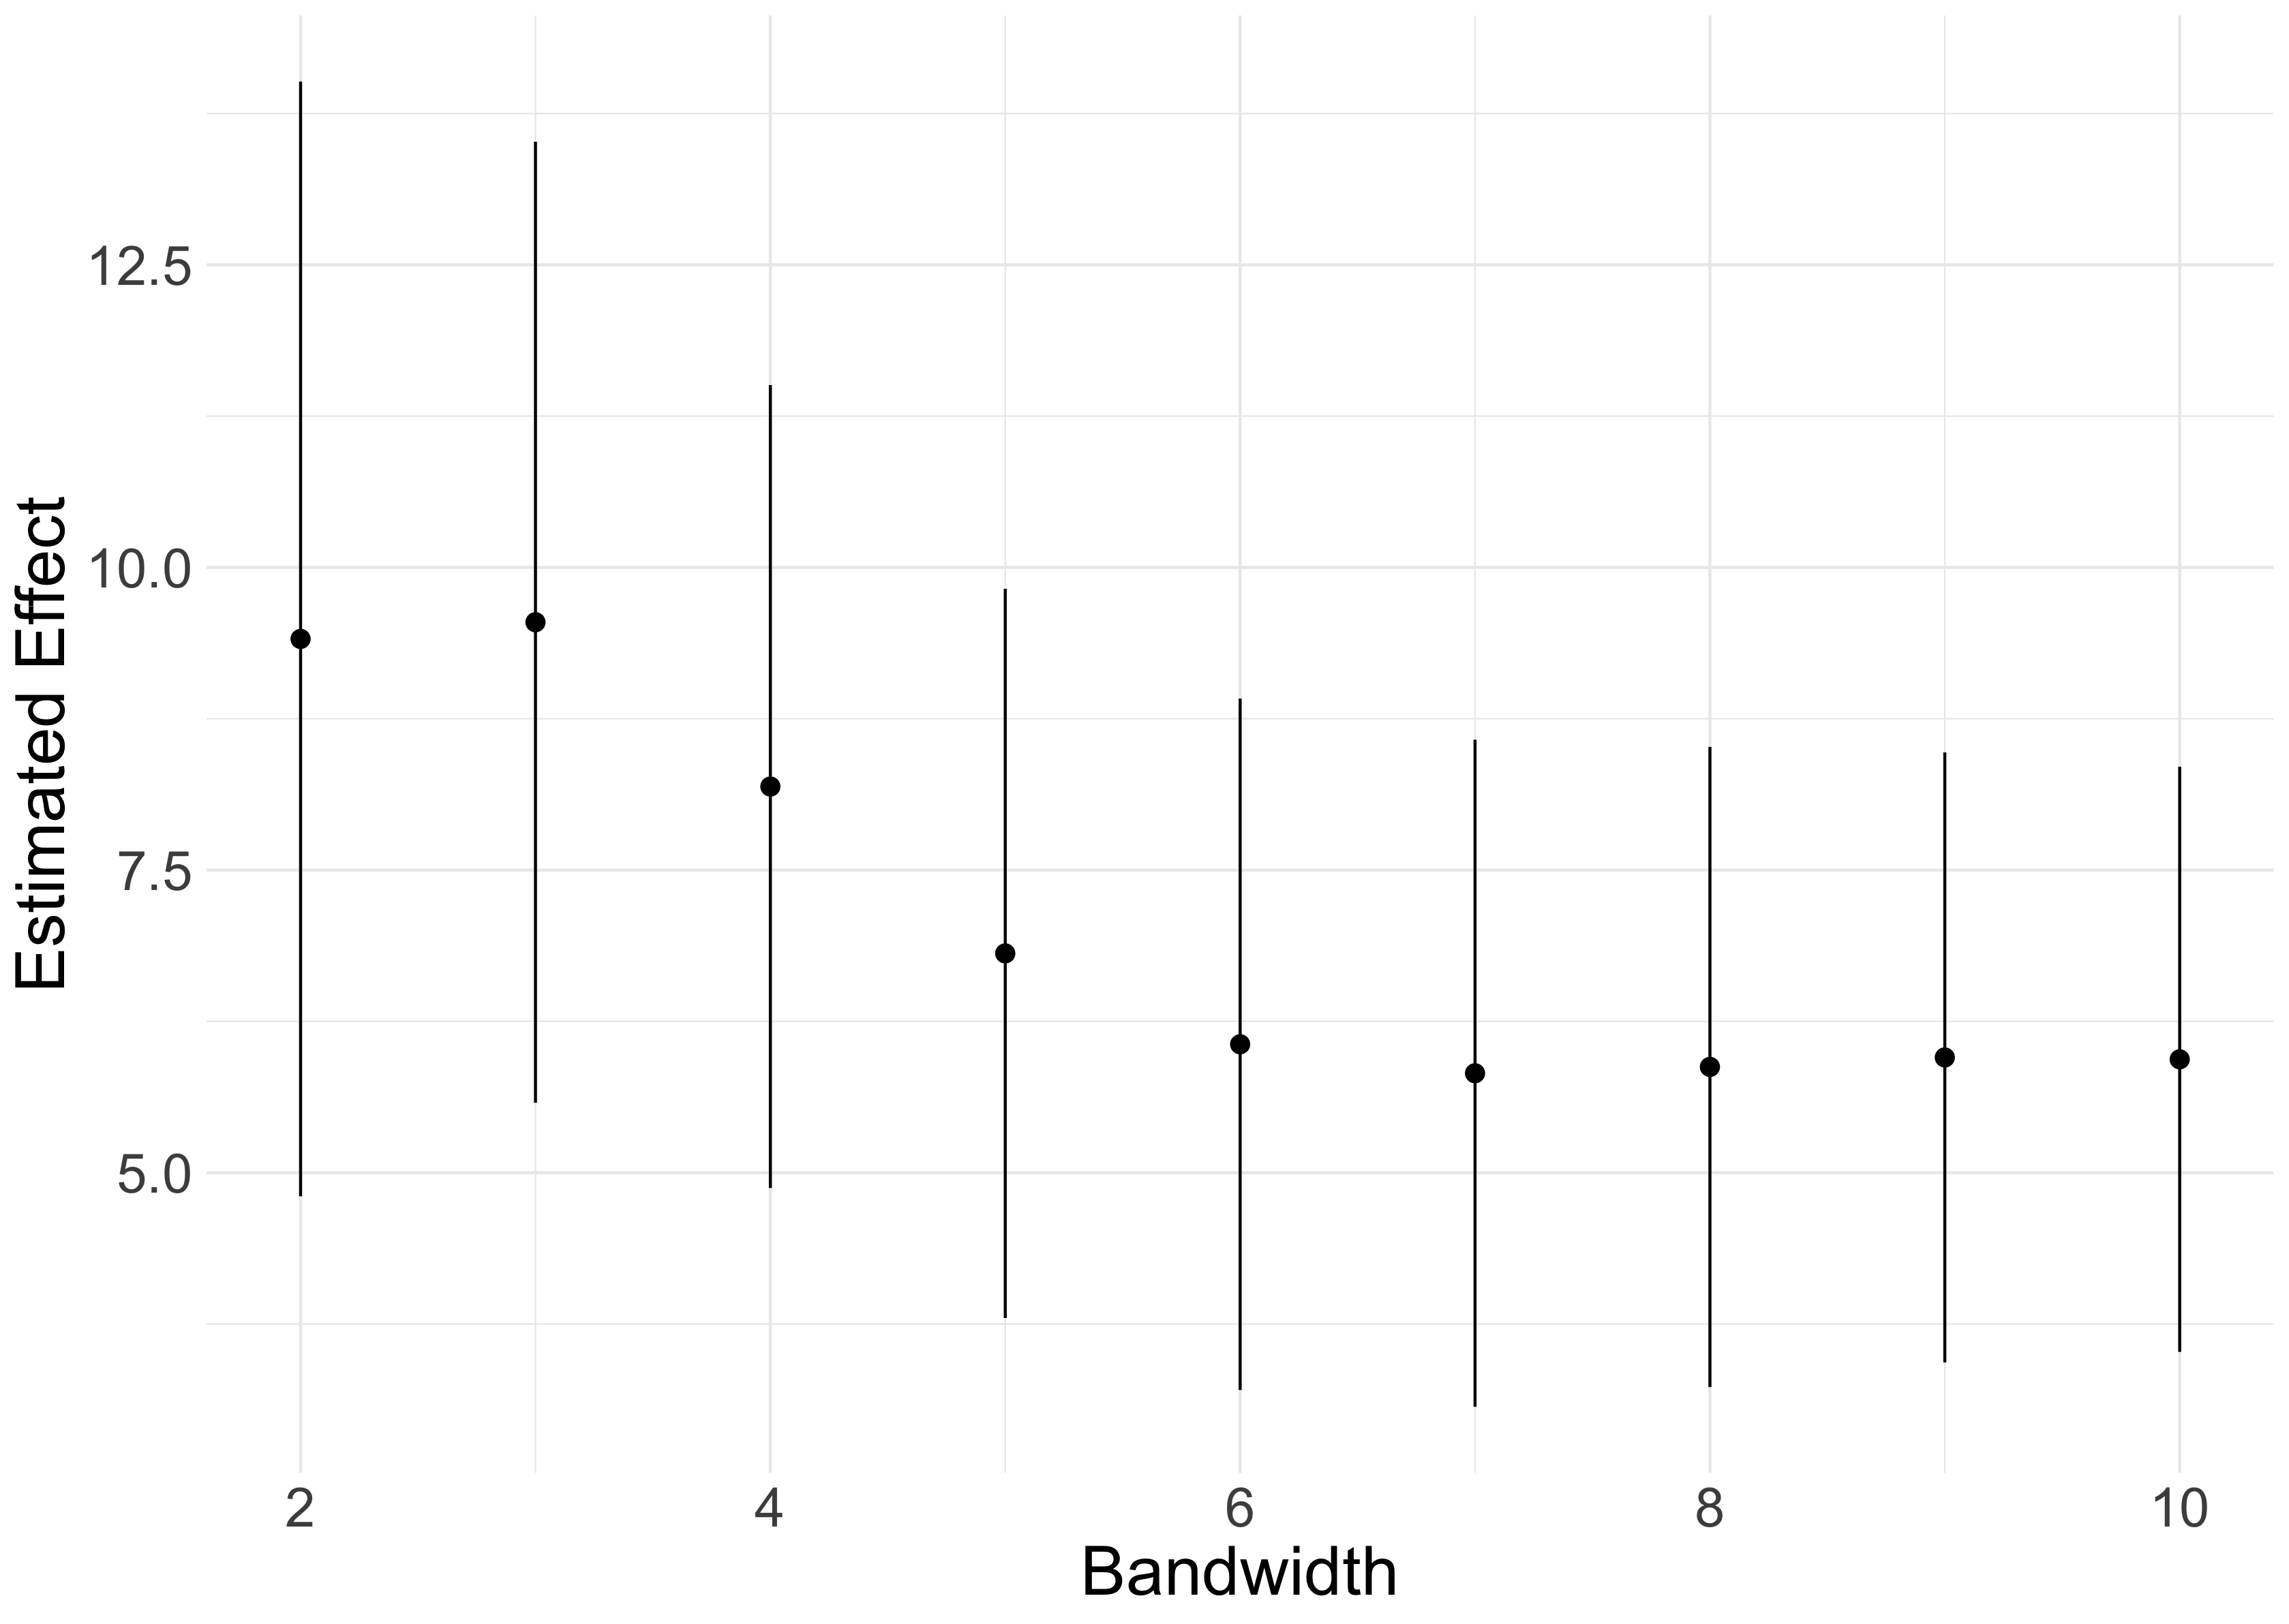
\includegraphics[width=\linewidth]{images/lee_rd_binscatter_output_robust.png}}                       \end{column}%
    \end{columns}
\end{frame}

\begin{frame}{Next time}
  \begin{wideitemize}
  \item Discrete RD
  \item Bias from RD estimation
  \item Regression Kink
    \item Bounds on treatment effects
  \end{wideitemize}
  
\end{frame}





\end{document}